\svnkwsave{$RepoFile: siminos/spatiotemp/chapter/blogMNG19.tex $}
\svnidlong {$HeadURL: svn://zero.physics.gatech.edu/siminos/spatiotemp/chapter/blogMNG19.tex $}
{$LastChangedDate: 2020-10-26 00:49:15 -0400 (Mon, 26 Oct 2020) $}
{$LastChangedRevision: 6799 $} {$LastChangedBy: predrag $}
\svnid{$Id: blogMNG19.tex 6799 2019-03-12 05:22:19Z mgudorf3 $}

\chapter{Matt's 2019 blog}
\label{chap:blogMNG19}
% Predrag                                           15 March 2019

\begin{description}

\MNGpost{2019-01-10}{
\begin{description}
\item[Paper on spatiotemporal defects]
Trying to put the finishing touches on the written document for my thesis proposal.
While sourcing some of my written statements I stumbled across something interesting
in \refref{witt99hol}, displayed in the quote,

\begin{quote}
We believe that the longer time scales for the excited modes arise from the metastability
of the cellular solutions (which are stable for small L) undergoing continuous creation
and annihilation events (``space-time defects'')\rf{ChowHwa95}
\end{quote}

It is \refref{ChowHwa95} that is the earliest reference to ``space-time defects'' that I have
found. The lion's share of the work presented is regarding wavelet-based simulation
as well as statistical computations but there are certain ideas that could possibly
be useful for my needs.

Both of these papers discuss spatial and temporal scales as well as reframe
dynamics in terms of ``metastable cellular solutions'', ``space-time defects'' and
in \refref{ChowHwa95} they reference the system (\KSe) being ``frustrated'' by the existence
of multiple ``metastable cellular states''.

I haven't delved too deep into either paper but on the surface it seems like there
is some low-hanging fruit that can be picked for spatiotemporal purposes.

\end{description}
}

\begin{figure}
\begin{minipage}[height=.3\textheight]{.32\textwidth}
\centering \small{\texttt{(a)}}
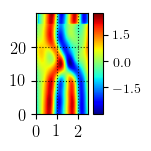
\includegraphics[width=1.0\textwidth,height=.25\textheight]{MNG_HOD_init}
\end{minipage}
\begin{minipage}[height=.3\textheight]{.32\textwidth}
\centering \small{\texttt{(b)}}
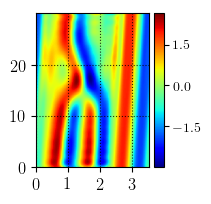
\includegraphics[width=1.0\textwidth,height=.29\textheight]{MNG_HOD_STREAK_init}
\end{minipage}
\begin{minipage}[height=.3\textheight]{.32\textwidth}
\centering \small{\texttt{(c)}}
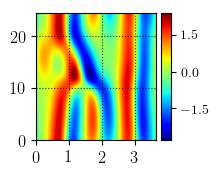
\includegraphics[width=1.0\textwidth,height=.17\textheight]{MNG_HOD_STREAK_final}
\end{minipage}
\caption{ \label{fig:MNGhodstreak}
(a) Initial condition from \reffig{fig:MNG_HOD_tile} that converges to
a solution that is believed to be a numerical continuation of (b) from \reffig{fig:MNGsymb11}. (b) An initial condition
resulting from concatenating a streak-pair with (a), that
numerically converges to (c).
}
\end{figure}

\begin{figure}
\begin{minipage}[height=.3\textheight]{.32\textwidth}
\centering \small{\texttt{(a)}}
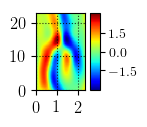
\includegraphics[width=1.0\textwidth,height=.25\textheight]{MNG_HD_init}
\end{minipage}
\begin{minipage}[height=.3\textheight]{.32\textwidth}
\centering \small{\texttt{(b)}}
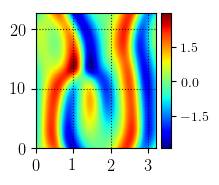
\includegraphics[width=1.0\textwidth,height=.29\textheight]{MNG_HD_STREAK_final}
\end{minipage}
\begin{minipage}[height=.3\textheight]{.32\textwidth}
\centering \small{\texttt{(c)}}
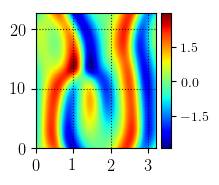
\includegraphics[width=1.0\textwidth,height=.17\textheight]{MNG_HD_STREAK_final}
\end{minipage}
\caption{ \label{fig:MNGhdstreak}
(a) Initial condition that has not been shown to numerically converge. (b) An initial condition
resulting from concatenating a streak-pair with (a), that
numerically converges to (c).
}
\end{figure}


\MNGpost{2019-01-18}{
In an attempt to restart the hunt for symbolic dynamics, some initial guess tiles
that were used in the frankenstein reconstruction efforts were used to attempt
to find more tiles. These by themselves did not numerically converge to \spt\ \twots\
but by concatenation of a single streak (crest trough pair) in space is necessary and
sufficient to numerically converge the solutions. I believe that this elucidates some
of the spatiotemporal symbolic dynamical grammar.

Let $0,1,2$ represent ``streaks'', ``defects'' and ``gaps'' family members, respectively.
If we assume that the subdomains ``half-defect'' and ``hook-on-top-of-defect'' correspond to
a 2-by-1 time by space symbolic dynamic chain,

\beq
\text{hook on defect} =
\begin{bmatrix}
  1 \\
  1
\end{bmatrix} \,,
\eeq

then this is believed to be inadmissible, but can be made to be admissible by conjoining
a streak spatially, which is believe to have symbolic representation,

\beq
\begin{bmatrix}
  1 & 0 \\
  1 & 0
\end{bmatrix}\,,
\eeq

Likewise, for the half-defect symbolic tile I believe the most accurate guess would be

\beq
\text{hook on defect} =
\begin{bmatrix}
  2 \\
  1
\end{bmatrix} \,,
\eeq

then this is believed to be inadmissible, but can be made to be admissible by conjoining
a streak spatially, which is believe to have symbolic representation,

\beq
\begin{bmatrix}
  2 & 0 \\
  1 & 0
\end{bmatrix}\,,
\eeq

which I believe gives an inkling into the possible grammar rules; my appeal to intuition
is that longer strings in time introduce instability which is balanced by introducing streaks
spatially as some kind of metastability.

These are demonstrated visually in \reffig{fig:MNGhodstreak} and \reffig{fig:MNGhdstreak}.

}

\begin{figure}
\begin{minipage}[height=.48\textheight]{.48\textwidth}
\centering \small{\texttt{(a)}}\\
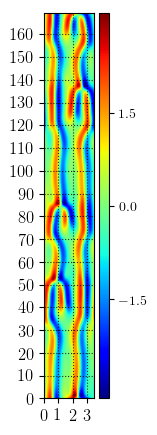
\includegraphics[width=.8\textwidth,height=.4\textheight]{MNGconvergedLR}
\end{minipage}
\begin{minipage}[height=.48\textheight]{.48\textwidth}
\centering \small{\texttt{(b)}}\\
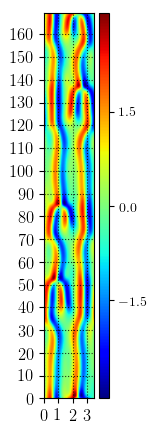
\includegraphics[width=.8\textwidth,height=.4\textheight]{MNGconvergedHR}
\end{minipage}
\caption{ \label{fig:MNG}
(a) \PPOtwot{21.94}{85.73} %\emph{ppo\_L21p94\_t85p73}
with a subdomain cutout, represented in (b). This
is a non-converged guess for what I title the ``half-defect''.
}
\end{figure}

\begin{figure}
\begin{minipage}[height=.48\textheight]{.48\textwidth}
\centering \small{\texttt{(a)}}\\
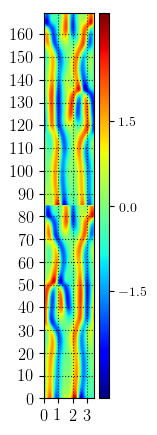
\includegraphics[width=.8\textwidth,height=.4\textheight]{MNGintegratedLR}
\end{minipage}
\begin{minipage}[height=.48\textheight]{.48\textwidth}
\centering \small{\texttt{(b)}}\\
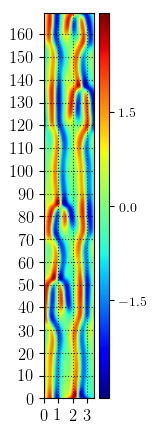
\includegraphics[width=.8\textwidth,height=.4\textheight]{MNGintegratedHR}
\end{minipage}
\caption{ \label{fig:MNG_halfdefect}
(a) \PPOtwot{21.94}{85.73} %\emph{ppo\_L21p94\_t85p73}
with a subdomain cutout, represented in (b). This
is a non-converged guess for what I title the ``half-defect''.
}
\end{figure}

\MNGpost{2019-02-04}{
Application of Hill's formula using the action functional defined by the integral of the
Lagrangian (density) previously derived in \refeq{eqn:KSLagrangian},
\beq
S[\phi] = \int \int \mathcal{L}(x,t,u,v,u_x,v_x,u_t,v_t,u_{xx},v_{xx}) dx dt
\eeq
yields a Hessian matrix whose determinant does not rely on the values of
either the original scalar field $u$ or the adjoint variable $v$. This is
due to the specific matrix structure, not due to absence of $u$ or $v$ as
matrix elements. Specificially, the matrix of second variations, or
Hessian of the action functional, is given by
\beq
\begin{bmatrix}
2v/3 & u_x/3 & 0 & -1/2 &v/3 & 2u/3 & 0 &0 \\
u_x/3& 0 & 1/2 & 0 & u/3 & 0& 0& 0\\
0    &1/2 &0 &0 &0 &0 &0 &0 \\
-1/2 &0 &0 &0 &0 &0 &0 &0 \\
v/3  &u/3 &0 &0& 0& &0 &0 &0 \\
2u/3 &0 &0 &0 &0 &0 &0 &0 \\
0    &0  &0 &0 &0 &0 &0 &1 \\
0    &0  &0 &0 &0 &0 &1 &0 \\
\end{bmatrix} \,.
\ee{NotHessian}
The determinant of this matrix is constant and equals $1/16$. The matrix elements are understood
to be shorthard for the spatiotemporal integral present in the action functional definition.
The constant determinant value has confused me for a
some time and I have been attempting to figure out if this makes any sense. The determinant
can be substituted into the expression
for Hill's formula from \refref{BolTre10} to yield,
\beq
\det(P-\mathbb{I}) = \sigma (-1)^m \beta/16 \,.
\eeq
For the \spt\ \KSe\ the dimension of the configuration space manifold $m=2$; the only comments
regarding $\beta$ and $\sigma$ are that they are a ``scaling factor'' and $\sigma = \pm 1$ ``takes care of
orientation''; that is the extent of their explanation. I'm unsure how to interpret this unless the ``scaling
factor'' is dependent on $u,v$. Also, the argument of stability of periodic solutions is predicated on the sign
of the RHS, so I believe it's determined \textit{a priori} by the fact that we know unstable solutions exist.

This result seems very artificial; I believe it is due to the artificial introduction of Lagrangian structure
for problems that originally had none. This lead me to investigate as much as possible if this formulation is
indeed worthless or not. Ibragimov\rf{Ibragimov07a} utilizes this ``formal Lagrangian'' to construct new
conservation theorems and conserved quantities for partial differential equations using Lie theory. Other
references refer to this type of construction as an ``extended Lagrangian''\rf{Kraus13}. Kraus claims that there is a
better alternative to Ibragimov's quasi self-adjoint derivations in terms of simplicity. Specifically, he claims that
if adjoint and or dual variables $v$ and its collection of partial derivatives (jet prolongation) can be chosen such that
the adjoint equation is satisfied when the \KSe\ is satisfied then the formal Lagrangian formulation is physically relevant.

\begin{quote}
``If it is possible to select the relation (2.286) such
that (2.287) is automatically respected when u solves (2.281), then a conservation law for
the extended system amounts to a physical conservation law.''
\end{quote}

In other words, the stationary points of the action are where the variational derivatives of the action are equal to zero.
For this Lagrangian formalism, this is equivalent to satisfying the adjoint equations and the \KSe\ simultaneously. This
is no where near obvious as it depends on the choice of adjoint variable \ie $v = \phi(x,t,u,u_{(1)}, ...)$.
Luckily, there is no reason to not choose the \KSe\ itself as the adjoint variable, even though it might seem tautological on the surface. Each term
in the adjoint equation is linear in $v$ and its derivatives; therefore, choosing $v = F(\tilde{\mathbf{u}})$ guarantees the criterion that
we want to guarantee.
While this does not explain whether or not the use of Hill's formula makes any sense, it is an argument that any conserved quantities derived
from the Lagrangian would be physically relevant. The justification from
\refref{Kraus13} is that being able to express $v$ as purely functions of the original
scalar field guarantees that symmetry of the extended ``formal Lagrangian'' system can be reduced to symmetries of the original system.
Sadly my (Lie) algebra skills need some work as I kept getting confused with what jet prolongation, the differences between Lie-B\"acklund and Lie point symmetries,
and how to produce the set of generators that span the Lie algebra and extend them to include the adjoint variables.
Once I derive the correct set of generators that span the Lie Algebra I should be able to derive something useful.

One proposed explanation is that technically due to doubly periodic boundary conditions, all Hessian matrix elements represent integrals,
which are technically zero. This leads to a very simple expression for the characteristic polynomial of the Hessian, the eigenvalues
are $\pm 1, \pm 1/2$ each with multiplicity $k=2$.

Although it is reaching, this might be a manifestation of the action functional being $\mathcal{P}\mathcal{T}\text{-symmetric}$, which
constrains the eigenvalues to be real. It is a weaker condition than the Hessian being Hermitian although technically by being real and symmetric
it is anyway. I really don't know how to explain this away so I've been attempting and failing to derive a conserved quantity that might be of future
use.
}

\MNGpost{2019-02-13}{
\begin{description}
\item[Lie groups and algebras for Lagrangian formalism]
The following will hopefully serve as both a report on what
I have been doing as well as a guide to refer back to.

While I haven't delved into the really mathematical formalism
(pullbacks,lifts,contact) there are a few preliminaries
that are absolutely essential to understand the description
that follows,

\begin{enumerate}
\item Jet prolongation\rf{KraMaj15,Kraus13} (sometimes referred to by
the constituent pieces: jets,prolongation, jet bundles)
\item ``formal'' or ``extended'' Lagrangians\rf{Ibragimov11}
\item  Lie algebras and their generators (sometimes referred to as vector fields
instead as the generators are differential forms that act on the relavant manifold)
\item Prolongation of Lie algebra generators
\item The difference between Lie point group operators and Lie-B\"acklund
operators.
\item Extension of generators to adjoint variables
\item Conserved vectors and conservation theorems
\end{enumerate}

The best single sentence I have found to describe jet bundles
and prolongations comes from \HREF{https://en.wikipedia.org/wiki/Jet_bundle}{Wikipedia}:
``Jets may also be seen as the coordinate free versions of Taylor expansions''.

Instead of ruining the discussion with words such as \emph{sections, fibre bundles,holonomic
sections, tangent lifts,etc.}, I'll merely define the $n$th jet prolongation
as a mapping that takes a set of independent and dependent variables, e.g.
$(x,t,u)$, and returns all derivatives with maximum order $n$:

\beq
j^{n}\psi \equiv j^{n}(x,t,u) = (x,t,u,u_x,u_t, ..., \frac{\partial u}{\partial x^{i_1}...\partial x^{i_n}}).
\eeq

The concept of formal Lagrangian was previously used to derive \refeq{eqn:KSLagrangian}.
Introduction of new dependent variables, ``adjoint variables'', $(v,v_x,v_t,...)$
can be used to impose a Lagrangian structure where there formally was none.
Accordingly, a Lagrangian that depends on both the original dependent variables
and their adjoints can be derived, such that the variational derivatives
reproduce the \KSe\ and its adjoint.

The infinitesimal generators of a Lie group are
vector fields which are elements of the Lie algebra. Each vector field
generates a one-parameter family of symmetry transformations.

These vector fields are usually written
as an expansion in terms of derivatives with respect
to independent $x^{i}$ and dependent variables $u^{\alpha}$,
%%%%%%%%%%%%%%%%%%%%%%%
\beq
\mathbf{X} = \sum \epsilon^{i} \frac{\partial}{\partial x^{i}}
+  \sum \eta^{\alpha} \frac{\partial}{\partial u^{\alpha}}
\eeq

If the coefficients in this expansion only depend on the independent
variables and the dependent variable (no dependence on derivatives), \ie,

\bea
\epsilon^i&=&\epsilon^i[x,t,u] \continue
\eta^j&=&\eta^j[x,t,u]
\eea

%%%%%%%%%%%%%%%%%%%%%%%
then the symmetries will be referred to as Lie \emph{point symmetries},
otherwise they will be referred to as Lie-B\"acklund symmetries.

This expansion, while commonly presented in this form, is rather misleading as it carries
an implicit assumption along with it; namely, that it needs to be
\emph{prolonged} to the highest order of derivative of relevance in order
to be correct.
For example in the \KSe, this would require a prolongation of order four,
due to the presence of fourth spatial derivative. The specific formula
for the coefficients of these additional differentials are sometimes
referred to as \emph{prolongation formula}. It requires (total)
differentiation of existing coefficients,
%%%%%%%%%%%%%%%%%%%%%%%%%%%%%%%%
\beq
\eta^{\alpha}_{J} = D_J ( \eta^{\alpha} + \epsilon^{i} u_i^{\alpha}) + \epsilon^{i} u_{(J,i)}^{\alpha}
\eeq

As previously mentioned, the specific form of the expansion is determined by the relevant PDE
and assumptions. This expansion together with the invariance condition,

\beq
\mathbf{pr} \mathbf{X}(F( j^n \psi )) = \mathbf{0 },
\eeq

%%%%%%%%%%%
produces a (typically overdetermined, at least for point symmetries)
system of equations that can be used to determine coefficients of
the corresponding infinitesimal generators that span the symmetry
Lie algebra.
This step always seems to be taken for granted or not displayed, as its
likely a lengthy symbolic pen-and-paper (also known as Mathematica) computation.

This isn't even the entire story for us, as the general expression
for the infinitesimal generators needs to be \emph{extended} to include
the terms corresponding to the prolongation of the adjoint variables.

If the symmetry Lie algebra is known, then the spanning operators
can be immediately extended to include the adjoint variables.
There are formulae for determining the coefficients of extension
terms depending on Lie point or Lie-B\"acklund symmetry is being considered.

In summary, symmetries or their equivalent generators are derived
by the prolongation of a general expansion to the PDE of relevance.
This and an invariance condition allows one to determine the coefficients
of the expansion and hence the generators that span the Lie algebra.

Once the generators have been derived, they are extended to include the
adjoint variables, yielding operators that can be used in conjunction with the \emph{conservation equations},
%%%%%%%%%%%%%%%%%%%%%%%%%%%%
\bea
D_i(C^i) &=& 0 \continue
C^i &=& \epsilon^i \mathcal{L} + W^{\alpha}[ \frac{\partial \mathcal{L}}{\partial u^{\alpha}}] - D_k \frac{\partial \mathcal{L}}{\partial u^{\alpha}_{ik}}]+D_k (W^{\alpha})\frac{\partial \mathcal{L}}{\partial u^{\alpha}_{ik}}
\eea

in order to produce conserved quantities.

A very relevant and important piece of information regards symmetries
and conserved quantities of the extended Lagrangian. Namely, \refref{Kraus13}
claims that if the adjoint equation is automatically satisfied
when the \KSe\ is satisfied, i.e. if $F^*(j^4(x,t,u,v))=0$
when  $F(j^4(x,t,u))=0$, then ``a conservation law for the extended system amounts
to a physical conservation law''. Also for the conservation laws
to be non-trivial, the extended equations need to be \emph{nonlinearly self-adjoint},
which is equivalent to the previous statement regarding the adjoint being satisfied
when the original equation is satisfied.


\item[KS Lie algebra]
I've been trying to do the symbolic computation with Mathematica
to derive the extended operators that span the Lie algebra but the
process has been slow because I'm not used to Mathematica and I've
found it very easy to lose my place amidst all of the indices.

Luckily, I feel more comfortable with the general procedure and
ideas that constitute what I suppose amounts to a Lagrangian field
theory. The entire point behind this exercise was to derive
interesting and relevant conserved quantities for the spatiotemporal \KSe,
i.e. to utilize the Lagrangian formalism as much as possible.

\end{description}
}

\MNGpost{2019-02-15}{
Notes from discussion with Lan.
\begin{itemize}
\item His first suggestion to get a better grasp on the spatiotemporal symbolic dynamics
is to plot spatiotemporal solutions in a phase space of higher dimension but similar to that
of \refref{DoLa14}. Specifically, plot partial derivatives $u_t, u_{tx}, ...$ as functions of
space and time and see how this space is organized. This might provide a smarter way forward
for determining the grammar.
\item His second comment is regarding troubles on the horizon concerning the continuous
families of solutions, one such worry is how to deal with boundary conditions of an infinite
domain.
\item Regarding the Hill's formula ``result'' using the formal Lagrangian, he thinks that
if true it's actually a great result because the continuous families are an indication of
a hidden symmetry, so if the solutions in these families all the same stability it would
be nice.
\item Regarding the Lagrangian itself, he believe it is a good theoretical attempt, and
thinks the theory is really the lion's share of the remaining work.
\item He's been thinking of this a lot and has a lot of his own ideas which we did not
get into but he believes that I've done really impressive work that has gotten him really
excited in regards to his ideas. It made me very happy and he even went so far as to say
``This is really important'' in regards to my work; not only for fluid dynamics but also for
chaotic systems and PDEs in general.
\end{itemize}

Hopefully this optimism leads to good results and many publications :)
}

\PCpost{2019-02-16}{
We'll have to teach Lan how to use GaTech VPN - lots of hoops to start with,
until it works. His GaTech ID is
\\
\texttt{lyueheng6 	Sp....t......l?}
\\
His subversion ID is\\
\texttt{y-lan       b.T......!}
}

\PCpost{2019-02-19}{
I have not really digested \refeq{NotHessian}, but a quick remark. For
for discrete time flows the Hessian of a \po\ is a high-dimensional
finite matrix, with every point on the cycle-$n$ varied (see Han's blog);
for continuous time flows it is an infinite matrix, that's why it took
\Poincare\ to prove that it's determinate is finite. So a single matrix
\refeq{NotHessian} is not the Hessian, or is a Hessian only for an \eqv\
solution?
    }

\MNGpost{2019-03-11}{
\begin{description}
\item[LSS Methods]
I've been reading the Least Squares Shadowing method developed in \rf{Wang14}
and mentioned in both \rf{LaShMe18,Lasagna17}. I had a former roommate explain
adjoint methods and their application in an engineering context. Typically from
what I have seen in adjoint methods is that engineers acknowledge that solving
for the full velocity field is hard so they write the adjoint equations such
that there are only a few control variables being varied instead of a very high
dimensional flow field. I believe this is because engineers are predominately
searching for stable equilibria by varying control parameters such as: airfoil
geometry, drag coefficient, etc.

I think I need to read the Lasagna papers more thoroughly to see how the LSS
method is applied to chaotic systems. I believe Wang's method only applies for
finding the derivatives of observables w.r.t scalar control variables, in my
case this would be the domain size, period, spatial shift (or energy, or another
conserved quantity yet to be discovered).

\item[Symbolic Dynamics]
Trying to get back into the swing of things by pursuing Lan's method
of plotting partial derivatives in order to develop some intuition regarding the admissible
spatial and temporal combinations of tiles in order to develop the symbolic dynamics.

I don't have anything worth showing really but I'm starting to believe that the spatial
itineraries might be decoupled from the temporal ones; I haven't really developed
an idea as to what is the best way to plot these yet, but following \rf{DoLa14}
and plotting in the $u,u_x$ plane and taking temporal cross sections of \spt\ \twots\
shows patterns similar to spatial equilibria ($T=0$ system). I believe this makes
sense as spatially conjoining two tiles means that each time instance must be periodic in space;
therefore I believe the intuition is something like follows: To glue two tiles $0$,$1$ spatially,
then at each instant in time the combination needs to be topologically equivalent to a spatial
equilibrium $01$. This is really hard to demonstrate other than rather vague attempts such
as the time dependent trajectory in $(u,u_x,u_t)$ space needs to intersect $(u,u_x,0)$ plane
to be able to glue spatially; this always seems to be the case so I believe a first
trial would be to continuously attempt to glue \eqva\ to an orbit and see if it can
be repeated ad nauseam. This could be misguided due to unwarranted projections, but
currently plotting trajectories as functions of space and time is far too obfuscating
to be useful. (similar to plotting trajectories prior to quotienting continuous symmetry
or plotting Fourier coefficients).

I believe this best way to proceed is to tile repetitively in space or time and then analyze the
corresponding partial derivative plots.

\end{description}
}

\MNGpost{04-04-2019}{
\begin{description}
\item[comments on Pathak \etal\rf{PHGLO18}]
{\em Model-free prediction of large spatiotemporally chaotic systems from
data: {A} reservoir computing approach}.
Slightly confused on what they mean by the ``echo state property" in their Fig.~1:
\begin{quote}
...all of the conditional Lyapunov exponents of the training reservoir
dynamics conditioned on $\mathbf{u}(t)$ are negative so that, for large
$t$, the reservoir state $\mathbf{r}(t)$ does not depend on initial
conditions.
\end{quote}
Is this a statement that the network is not being trained
w.r.t. transient behavior but rather trained by the attractor and or inertial manifold?

My main reaction to this paper is that it once again points
out how attached researchers are to the concept of time, and predictions of future behavior. They demonstrate that
after a small number of Lyapunov times that their predictions become inaccurate; while the predictions extend
past a few Lyapunov times I cannot help but think they
would be much better off training their reservoir on \twots\ so that the process isn't so much as predicting the
future as it is about "facial recognition" for lack of a better term. My bias is showing, but if they themselves acknowledge that there are fundamental limits imposed by
positive Lyapunov exponents I can't help but feel that it would be better to (even at different system size) develop a database of \twots\ and then find the "average" much like
how the "average" facial structure can be produced for different countries and ethnicities; in this sense one would develop averages for observable quantities, but, like
I stated, this is spatiotemporal bias.

\item[Least Square Shadowing]
Finally got around to rereading this thoroughly. I believe that we
originally investigated the Least Squares Shadowing (LSS)
\refrefs{Wang14,Lasagna17,LaShMe18} as a means of classifying continuous
families of solutions generated by dependence on system parameters $T,L$.
From what I have gleaned from these papers the LSS method has an
underlying engineering spirit I believe. It's a numerically stable means
to see how observable quantities change in response to changing system
parameters over both individual orbits and the attractor they shadow. I
believe the application to the control problem in \rf{Lasagna17}
regarding the \KSe is simply introducing a Lagrange multiplier and then
analyzing how observable quantities are sensitive to perturbation in this
multiplier.

It's good work but I don't think that it can be leveraged for my own work unless it would be decided that the desirable representative from each continous family has a minimized/maximized sensitivity to changes in $T,L$. I don't see any basis for this reasoning however.

\item[Partial derivative plotting and symbolic dynamics]
The intuition from the \KSe\ on the $T=0$ line from Dong and
Lan\rf{DoLa14} doesn't seem to extend to the spatiotemporal case; in
other words, there doesn't seem to be a useful projection onto partial
derivatives of the velocity field ($u,u_x,u_{tx}$, \etc.) that elicits
interesting behavior.

The way this idea was tested is as follows: For each tile, and each
projection axes, the respective fields ($u(x,t)$ and its partial
derivatives) were plotted for all values of $x,t$. If shadowing were
present, then it should be present three dimensional projection is how I
was thinking.

This doesn't seem to be the case; therefore, unless there
is some new development I'm ceasing this activity.

\item[Slowly learning Julia]
I'm starting to board the Julia train lead by conductor Gibson. I enjoy
how it's really tailored to scientific computing by not messing around
with object oriented programming, not to mention the fact that it's very
fast if programmed correctly. The problem is at this stage it seems that
in order to leverage the capabilities one would have to either create
wrappers for underlying C++ and Fortran codes or borrow them from other
projects such as \texttt{DifferentialEquations.jl}, so I'm not sure how
much independence I would have; my thoughts were to rewrite
\texttt{kstori2} in Julia before writing anything new but I'm unsure if
it is worthwhile at this stage. TL;DR I'm interested in pursuing this but
it's low on the priority list right now.

\end{description}
}

\MNGpost{04-09-2019}{:
\begin{description}
\item[variational methods and numerical implementations]
(Description of spatiotemporal problem, function defined.)
\begin{itemize}
\item define cost function (functional eqn.)
\item adjoint equations
\end{itemize}

\item[tile extraction]:
\begin{itemize}
\item decide on subdomain that we believe is suitable candidate.
\item retrieve the numerical subdomain, discretization and parameters
\item put through same code that found the
source torus
\item if converge, done
\item if not converge, take larger subdomain and repeat process iteratively or quit
\end{itemize}

\item[gluing]:
\begin{itemize}
\item two known solutions
\item interpolate onto fine discretization
\item aspect ratio
\item if continuous symmetry, rotate
\item if discrete symmetry, chop
\item numerically zero pad between boundaries
\item fill in with convex combinations of the boundaries of zero-padded region
\item convex combination isn't differentiable; know \KSe is smooth,
therefore perform filtering / smoothing / Fourier truncation
\item Coarsen discretization depending on numerical method used
\end{itemize}

\end{description}
}

\MNGpost{2019-04-22}{
Mainly been writing daily activities in \refsect{sect:GuBuCv17blog}~{\em
GuBuCv17blog.tex}, see posts there for changes.
\begin{description}
\item[Wei and Wang (2019) article]
The following passage consists of outtakes from Wei and Wang\rf{WeiWan19}.

Work studies dissipative Dullin-Gottwald-Holm (DGH)
equation using Lie symmetry analysis \`a la Ibragimov\rf{Ibragimov11}.

The DGH equation
\beq \label{e-DGH}
u_t - \alpha^2 u_{xxt} +ku_x+3uu_x
+\gamma u_{xxx} =
\alpha^2 (2u_x u_{xx} +u u_{xxx})\,.
\eeq
results from
\begin{quote}
\textit{``...using asymptotic expansions directly in the
Hamiltonian for Euler's equation in the shallow water regime.
It is completely integrable with a bi-Hamiltonian as well
as a Lax pair...''}
\end{quote}

The equation that is referenced far more
often than the general Dullin-Gottwald-Holm equation
is the special case
\beq \label{e-NovruzovDGH}
u_t - u_{xxt}+3 u u_x
- 2u_x u_{xx} - u u_{xxx}
+k(u+u_{xx})_x+\lambda(u-u_{xx})=0\,.
\eeq
{\color{red}
(which is quite clearly the center
of the study of this paper)}
from \rf{Novruzov13,NovHag14}.  The title and
abstract are slightly misleading as the
general case is \emph{not} the emphasis of the study.

Certain parameters values
$k=\lambda=\gamma=0$, $\alpha^2=1$ produces the \emph{Camassa-Holm} equation
\beq \label{e-CH}
u_t - u_{txx} +3uu_x
+u_{xxx}-2u_x u_xx-u u_{xxx}=0\,,
\eeq
which describes ``unidirectional
propagation of surface waves on a shallow
layer of water that is at rest at infinity.''

Wei and Wang then discuss Ibragimov's \textit{formal Lagrangian} formalism%
\rf{Ibragimov07b,Ibragimov11,Ibragimov18}
as well as the nonlinear self-adjointedness
property\rf{Ibragimov07b,Ibragimov11}.
    \PC{2019-04-22}{Here Matt referred to \emph{Ibragimov10}, I cannot find it.}

Very briefly, the main concept at hand is
that by creating a formal Lagrangian
$\mathcal{L}=vE$ where $E$ is an $s$-th order
nonlinear equation (e.g. the DGH equation or the \KSe).
An equation that is nonlinearly self-adjoint has the property that the
adjoint equation
\beq \label{e-formaladjoint}
E^*=\frac{\delta \mathcal{L}}{\delta u}=0 \,,
\eeq
is satisfied by some substitution $v=\phi(x,u)$.
Here, $\delta$ signifies the variational derivative
(many different names, see the ``Names'' section
of \HREF{https://en.wikipedia.org/wiki/Material_derivative}{Wikipedia}).

Written more explicitly, the nonlinear
self-adjoint condition can be written
\beq \label{e-nonlinearadjoint}
E^*\Big|_{v=\phi}=\lambda_0 E+\lambda_1D_t E+\lambda_2D_xE + ...
\eeq
where $\lambda_i$ depend on $u$ and its derivatives.

\MNG{
If the ``extended system'' (the variational
derivatives) satisfy
$\frac{\delta \mathcal{L}}{\delta u}=\frac{\delta \mathcal{L}}{\delta v}=0$
for some $v$ (\ie is nonlinearly self-adjoint)
any conservation law of the extended system
corresponds to a physical conservation law \rf{Kraus13}.
}

{\color{red}
The point that frustrates me to no end, maybe I'm just ignorant,
is that the symmetry operators admitted by the equation are stated
without derivation.
By ``the'' symmetry operators of an equation
I mean the set of operators which
leave the equation invariant as well as produce the Lie algebra. The machinery
developed by Ibragimov is
\emph{completely reliant on the derivation of these generators, or worse, having a priori knowledge}.
For example, the following Lie point symmetry
operators admitted by \refeq{e-NovruzovDGH}
\beq \label{e-NovruzovDGHpointsymm}
X_1=\partial_t,\: X_2=\partial_x\: \text{and}\: X_3 =e^{\lambda t}(\partial_t +k\partial_x -\lambda u\partial_u)\,.
\eeq
I understand the inclusion of the generators of translations, $X_1$ and $X_2$,
but have \emph{absolutely no idea} why they include $X_3$ without derivation as it seems
very non-trivial to me. I \emph{believe}
it comes from the invariance condition
\beq
X_{\alpha}E = 0\,,\; \text{ where}\: X_{\alpha}
            = \xi_{\alpha}^{t}\frac{\partial}{\partial t}
             +\xi_{\alpha}^{x}\frac{\partial}{\partial x}
             +\eta_{\alpha}\frac{\partial}{\partial u}
\,,
\eeq
which produces an over-determined linear system of equations wherein the coefficients
$\xi_{\alpha}^{t},\xi_{\alpha}^{x},\eta_{\alpha}$ of generators $X_{\alpha}$ are
determined by solving said system of equations.
}
Moving beyond this point of contention,
they state that ``...optimal system of one-dimensional subalgebras
of the Lie algebra spanned by $X_1$,$X_2$,$X_3$ of \refeq{e-NovruzovDGH} given by..."
\beq
X_1,\: X_2,\: X_1+aX_2,\: \text{and}\: X_2+bX_3\,.
\eeq
Again, producing the generators is the
component I have had trouble with; perhaps
it is because I was trying to derive the generators for Lie-B\"acklund symmetries
because I did not have success with the easier case which is Lie point symmetries.

\MNG{The difference between Lie point symmetries and
Lie-B\"acklund symmetries (according to Ibragimov)
is whether the generators of the vector field (Lie algebra)
depend on the partial derivatives of $u$ (Lie-B\"acklund symmetry)
or not (Lie point symmetry).}

The rest of the paper, although not trivial,
follows the Ibragimov's blue print pretty
closely. The applications and derivations
include:
\begin{itemize}
\item Using nonlinear self-adjointedness
and Ibragimov's conservation theorem
\rf{Ibragimov07a} to derive conservation
laws for \refeq{e-NovruzovDGH}
\item Using conservation laws to show
solutions exhibit blow-up and the ``global
existence of strong solutions''
\item Deriving analytic solutions from the
conservation law
\end{itemize}

Details are left in the paper as the
proofs and derivations are too specific to
\refeq{e-NovruzovDGH} to be of use in the spatiotemporal \KSe.

\end{description}
}

\MNGpost{2019-04-23}{
\begin{description}
\item[Tom Day]
Graduate student from Peter Yunker's group presented on the manner
in which yeast forms clusters. This was motivated by the evolution
from single cell to multicellular organisms, want to investigate the
key properties of one such evolutionary process. The general idea is that
yeast cells will collect and subsequently undergo a budding process which creates
branches which result in large clusters. There were two differing
experimental setups which both resulted in the same mass distribution
as a function of cluster diameter. The general idea
was to have a tube consisting of a yeast mixture where after a set amount of time the bottom
portion (clusters stratify based on mass, bottom has largest clusters) was extracted.
Repeating this process iteratively
is equivalent to selecting the largest. It was shown
that the cells evolve by elongating (aspect ratio changes)
to improve packing efficiency. The distribution of cluster sizes
was only investigated for a finite period of time; nothing said about
the expected limits of such a process or whether there is a critical size
which clusters cannot exceed.

The two experiments both involved repeated extraction of the largest clusters, with
one critical difference. For one of the setups the yeast mixture was compressed at constant
force for a set amount of time prior to every extraction. In spite of this compression, the
distribution of the cluster sizes were identical. A model was created that related the
probability for the size to change by a scalar to the ``kinetics'' or rate which the
the clusters form. The model was based on some well known evolutionary model which
had structure similar to Boltzmann distribution. There was no link between this
model and experimental results sadly so it is not known whether the model is valid.

\item[Jaemin Park]
\textit{On radial symmetry of uniformly rotating stationary solutions}
\textbf{TL;DR for 2D Euler equation there is a (constant) range of angular velocities
where radially symmetric solutions exist. For the gSQG equation
there exists a similar range but it depends on a parameter (domain size I think?).}

Symmetry of \reqva\ and \eqva\ solutions to 2D euler. Using
vorticity equations and stream function formulation.
Biot-Savart law, Yudovich Theorem for uniqueness of weak solutions.
Vortex patch solutions, where the vorticity field is given by
linear combination of some functions.

The uniformly rotating patch with angular velocity
$\Omega$ counter-clockwise satisfies
\beq
z_t(t,\alpha) = \Omega z(t,\alpha)^{\bot}
\eeq
Boundary equation is the difference of the gradient
of the stream function minue the equation for $z_t$
dotted with some z.

Vortex patch is ``uniformly rotating'' if
\beq
\phi(x)-\frac{\Omega}{2}|x|^2=\text{Const}
\eeq
on each connected component of the boundaries.
Call this constant function $f(x)$.
If $\Omega=0$ then $\omega$ is a stationary solution.
Any radial solution is a rotating solution with
any angular velocity.

Question to be answered: Among all connected patches
with smooth boundary, must every rotatting patch with
$\Omega\leq 0$ or $\Omega \geq 1/2$ be radially symmetric?

Kirchoff (1876) showed than an ellipse is a rotating
solution where semi-axes satisfy
\beq
\Omega =\frac{ab}{(a+b)^2}
\eeq
two other statements, going too fast to type.
Theorem by the authors of the paper,
radial symmetry is broken in the parameter
range $0\leq \Omega \leq 1/2$.

Energy functional

\beq
1/2 \int p(x)(p\star \mathcal{N})(x)dx - \Omega /2 \int p(x)|x|^2 dx
\eeq
note that
\beq
\frac{\delta E}{\delta p} = f = \phi - \Omega /2 |x|^2
\eeq
Perturbations for a diveregence free vector field $V$ satisfy
continuity equations ``...''

Time derivative (inserting continuity equations) of the energy functional
implies that
\beq
\frac{dE}{dt} = \int V\cdot \nabla p = 0
\eeq

For an integral $\mathcal{I}$ that has a long definition, can show that
inequalities  only hold if patch is a disk for $\Omega \leq 0$ and $\Omega \geq
1/2$ as previously stated.

Putting holes in the patches betray the constraint $\mathcal{I}=0$;
need constant values of $p$ on boundaries.
Can bound a sequence of integrals (step functions) approximating
stream functions by isocontours of vorticity $\omega$ below by
some integral expressions, even though the limit of this quantity is zero.

Theorem; there exist stationary nontrivial patch solutions
to the 2D Euler equations even with finite energy.
These solutions are ``close'' to nested annuli with vorticity
of different sign. Proof bases on Crandall-Rabinowitz theorem.

Now consider Generalized Surface Quasi-Geostrophic equation.
Shown in literature the existence of non-radial solutions
in parameter range.

Difference between Euler and this is that the parameter range
where simply connected patches must be radially symmetric:
Euler has constant range, gSQG depends on the size of the domain.
Perturbation of the energy functional under ``continuous Steiner
symmetrization''.  ``Similar technique has been used to show
radial symmetry of steady solutions to nonlinear aggregation-diffusion
equations''.

Description of continuous Steiner symmetrization. Assume non symmetric patch,
split half-plane in two to split the
patch in two. Define ``needles'' (1D cross sections); make them symmetric
with respect to the half plane seperatrix.

Future work. Euler equation in unit disk.
``Can we still prove the radial symmetry of stationary patches on
the disks or annuli?''. Kirchoff ellipse solution (rotating solution).
Should be $0\leq \Omega << 1$ such that aspect ratio is very large (or small).
In other words, the future work is to investigate the parameter ranges
$0< \Omega << 1$ and $0< 1/2-\Omega <<1$.

``n-fold symmetric patch'' exist which look like smoothed polygons
which have $D_n$ symmetry.
\end{description}
}

\MNGpost{2019-04-24}{
My intentions for future edits of the paper; general
additions like including figures and citations are left out
in favor of more explicit goals.

Others would know better than me, but my gut is telling me that
if the paper is titled ``Spatiotemporal tiling of the \KS\ flow''
then incorporating Gutkin and Osipov is consistent with this message.
I foresee this process unfolding in two ways:
1. The paper is aimed at the overarching topic of spatiotemporal tiling,
for example, ``Spatiotemporal tiling of both discrete and continuous nonlinear
dynamical systems'' and the computational details such as adjoint method, GMRES,
etc. are left to another, more technical, paper.
2. The focus of the paper is the \KSe\ and the methods with which new solutions
have been found and can be constructed. This would go over the specific numerical
methods for finding solutions as well as gluing and tiling. I don't think \spt\
cats fits into this message personally.

For the second option I propose the following outline for the paper
\begin{enumerate}
\item Abstract
\item Intro
\item \KSe\ literature review
\item \Spt\ \KSe\ in Fourier basis (\texttt{sFb.tex})
\item \Spt\ symmetries
\item \Spt\ symbolic dynamics concept
\item Descent methods
\item Iterative methods
\item Gluing methods
\item Tiling methods
\item (If possible) symbolic dynamics quantitatively explained
\item Conclusion
\end{enumerate}
with the following reserved for appendices of either the paper or
thesis
\begin{itemize}
\item Variational methods
\item Matrix-free computations
\item Preconditioning
\item Fourier transform conventions and selection rules
\end{itemize}
with the caveat that if the Ibragimov-type study pans out, then
the results would be moved to the variational methods section which
would in turn be inserted between symbolic dynamics concepts and
descent methods. This is the narrative that I believe has the most
continuity. There is not much application of discrete Lagrangian methods
similar to \refref{KraMaj15}. While I believe this work is formulated
as a variational problem, almost all of the key components of discrete Lagrangian
methods are missing. For example, we do not formulate discrete jet bundles, discrete
action principles, discrete Noether's theorem, etc. These results are inherently
different from our calculation because they work in a discretized configuration
space $(x,t)$ and define everything in terms of finite differences on these
grid points.

The second option is more akin to how I believe my thesis will be structured
and so I am biased to approve of this format more. Due to the already
exorbitant length of \texttt{GuBuCv17.tex} I think that actually there
should be three papers: A \spt\ cat paper, a \spt\ \KS\ paper, and a
``grand narrative'' paper which builds on the results of the first two.

}

\PCpost{2019-05-13}{
I have already discussed it elsewhere, in {\bf 2019-02-26} post above, but it has
to go into the paper.

In \reffig{f:MNG_largeLtrans} and following figures,
the most unstable wavelength $2\pi\sqrt{2}$ of the u=0 \eqv\ (see
\refsect{sect:KSu0equiT}) is an estimate the mean spatial wavelength of
the turbulent \KS\ flow, so there are approximately 55 wiggles across the
spatial domain at any instant in time.
There is a very prominent leftward /
rightward wave propagation speed, perhaps several. But the result is
puzzling: on the left half, there are prominent leftward moving reddish
lines - but there are no prominent rightward moving bluish lines. Also,
both figures reveal a very persistent structure (not in our alphabet?)
from $(\conf,\zeit) = (9,0)$ to $(10,130)$ with a smaller wave velocity.
% (note, the \conf-axis is mislabelled).

If you look at \reffig{f:MNG_largeLtrans}, it has bluish regions and reddish
regions, and $u\in\{-3.4,+3.4\}$. But if you look at your (over-counted)
alphabet \reffig{fig:MNGtiles},
it has $u_j\in\{-2,+2\}$. Why is that?

You use Galilean invariance \refeq{GalInv} to set the mean velocity of
the overall front to zero,
\(
\spaceAver{u}(\zeit)
  \,=\, \int_0^{\speriod{}} d\conf \, u(\conf,\zeit) = 0
\,.
\)
But for an arbitrary subregion of width $\speriod{1}< \speriod{}$, the
mean velocity is generically $\spaceAver{u}(\zeit)\neq0$. Actually, we
know that as function of $\speriod{}$ the velocity front executes a
random walk, with variance
$E(\zeit)=\half\spaceAver{u^2}(\zeit)\propto\speriod{}$ by the
extensivity of \KS, and hence the range of the color bar in a figure such
as \reffig{f:MNG_largeLtrans} has to grow proportionally to
$\sqrt{\speriod{}}$. The variance grows only in the spatial direction, in
the time direction $E(\zeit)\to{E}$.

However, I think that if you plot $u_x$ for \reffig{f:MNGs_largeL} or
\reffig{fig:MNGtiles}, that might have bounded variance, as
$\spaceAver{u_x}(\zeit)$ is invariant under the $u(\conf,\zeit)\to
u(\conf -c\zeit) -c $ transformation.

That implies that in gluing letters $u_j$ of alphabet
\reffig{fig:MNGtiles} into larger patterns, one also has to vary
$\spaceAver{u_j}(\zeit)$ averaged over the tile of width $\speriod{j}$,
in order to glue optimally. In other words, we have to use the Galilean
symmetry group orbit of the letter $u_j$, and slice that group orbit at
$\spaceAver{u_j}(\zeit_0)=0$ for purposes of ploting its representative
in  \reffig{fig:MNGtiles}.

Perhaps the variational descent takes care of
that, but it is not obvious.
}

%%%%%%%%%%%%%%%%%%%%%%%%%%%%%%%%%%%%%%%%%%%%%%%%%%%%%%%%%%%%%%
%\begin{figure}[t]
%\begin{minipage}[height=.48\textheight]{.48\textwidth}
%\centering
%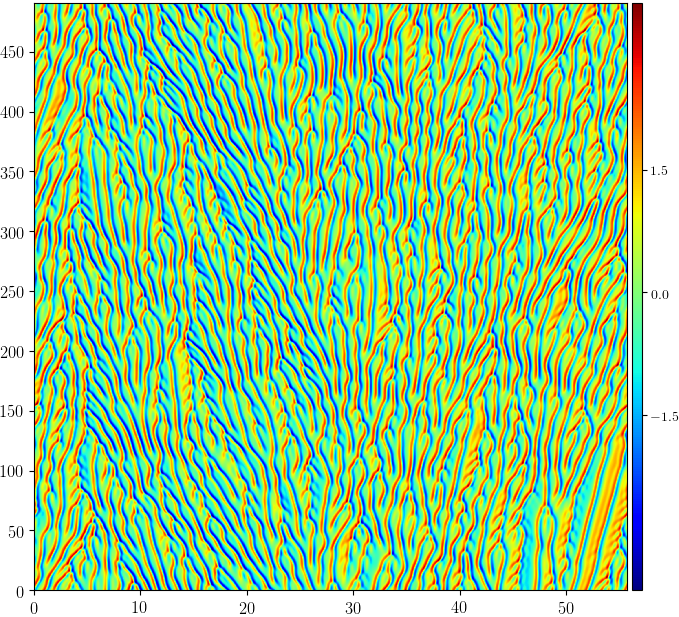
\includegraphics[width=1.0\textwidth]{MNG_u_largeL}
%\\ \small{\texttt{(a)}}
%\end{minipage}
%~~~~
%\begin{minipage}[height=.48\textheight]{.48\textwidth}
%\centering
%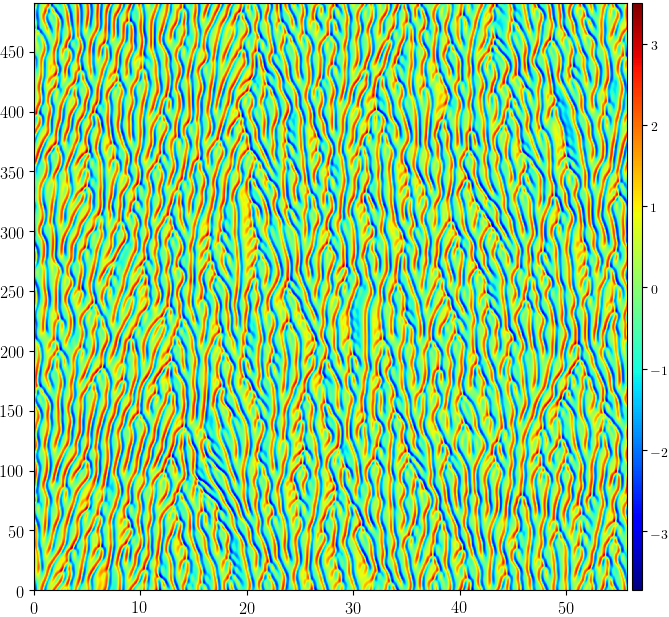
\includegraphics[width=1.0\textwidth]{MNG_u_largeL2000}
%\\ \small{\texttt{(b)}}
%\end{minipage}
%\caption{\label{f:MNG_largeLtrans}
%On dangers of peculiar initial conditions. Matt apparently started this simulation
%in a symmetric subspace.
%(a)
%A transient {\spt} \KS\ solution $u(\conf,\zeit)$,
%integrated forward in time on a spatially periodic domain of width
%$\speriod{}=500 \approx 55 \times 2\pi\sqrt{2}$
%(after a short time transient $\period{} \approx 50$). The blue
%stripe in the left half suggest very long time correlations,
%and there is pattern in the lower right corner never seen in any other simulation.
%(b)
%A typical {\spt} ``steady state turbulent'' \KS\ solution $u(\conf,\zeit)$,
%integrated forward in time on a spatially periodic domain of width
%$\speriod{}=500 \approx 55 \times 2\pi\sqrt{2}$
%(after a long time transient $\period{} \approx 2\,000$).
%The color bar indicates the color scheme for $u(\conf,\zeit)$, used also
%for the subsequent figures of this type.
%     }
%\end{figure}
%%%%%%%%%%%%%%%%%%%%%%%%%%%%%%%%%%%%%%%%%%%%%%%%%%%%%%%%%%%%%%%%%%%

%%%%%%%%%%%%%%%%%%%%%%%%%%%%%%%%%%%%%%%%%%%%%%%%%%%%%%%%%%%%%%
%\begin{figure}[t]
%\begin{minipage}[height=.48\textheight]{.48\textwidth}
%\centering
%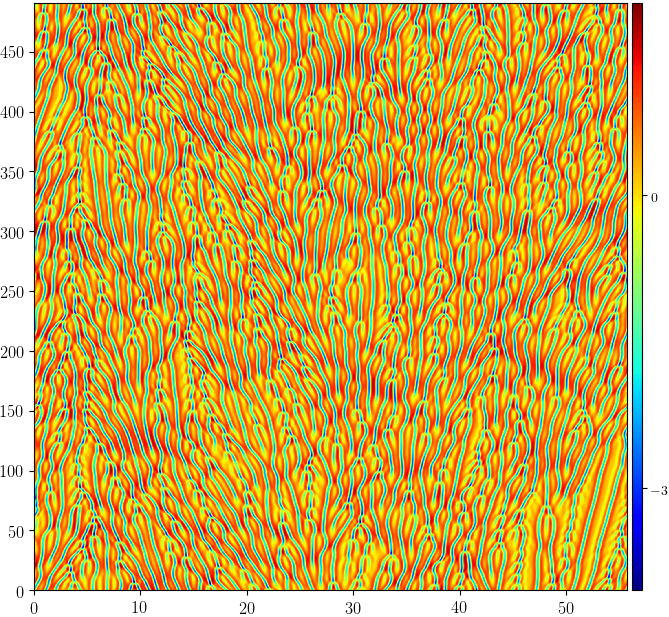
\includegraphics[width=1.0\textwidth]{MNG_ux_largeL}
%\\ \small{\texttt{(a)}}
%\end{minipage}
%~~~~
%\begin{minipage}[height=.48\textheight]{.48\textwidth}
%\centering
%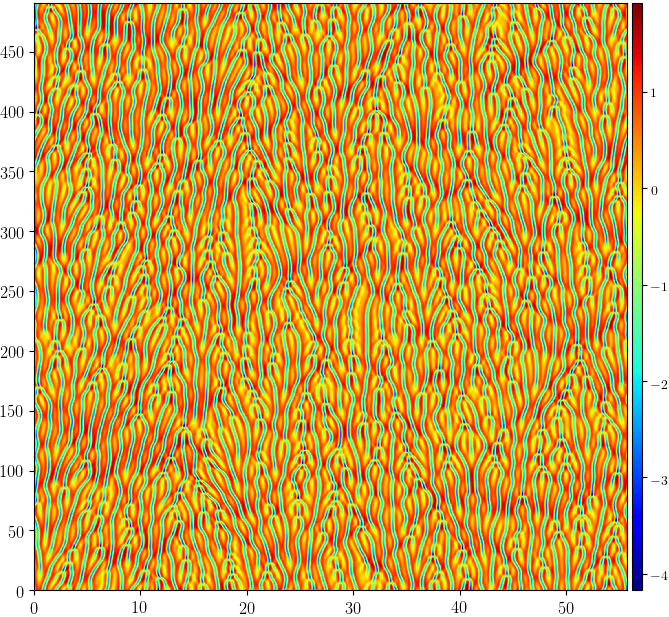
\includegraphics[width=1.0\textwidth]{MNG_ux_largeL2000}
%\\ \small{\texttt{(b)}}
%\end{minipage}
%\caption{\label{f:MNG_ux_largeLtrans}
%On dangers of peculiar initial conditions.
%(a)
%A transient {\spt} \KS\ solution, transient time $\period{} \approx 50$:
%the first spatial derivative $u_\conf$.
%(b)
%A typical {\spt} ``steady state turbulent'' \KS\ solution $u_\conf(\conf,\zeit)$,
%after a long time transient $\period{} \approx 2\,000$).
%The first spatial derivative $u_\conf$
%is a Galilean-invariant field, so it does not
%exhibit the random walk in its magnitude along the $\conf$ direction. It
%is interesting that the negative fluctuations of $u_\conf$ are much
%larger than the positive ones. In contrast, for $u$ we have parity symmetry
%\refeq{KSparity},
%$\spaceAver{u}(\zeit)= \spaceAver{\Refl \, u}(\zeit)$.
%     }
%\end{figure}
%%%%%%%%%%%%%%%%%%%%%%%%%%%%%%%%%%%%%%%%%%%%%%%%%%%%%%%%%%%%%%%%%%

%%%%%%%%%%%%%%%%%%%%%%%%%%%%%%%%%%%%%%%%%%%%%%%%%%%%%%%%%%%%%%
%\begin{figure}[t]
%\begin{minipage}[height=.48\textheight]{.48\textwidth}
%\centering
%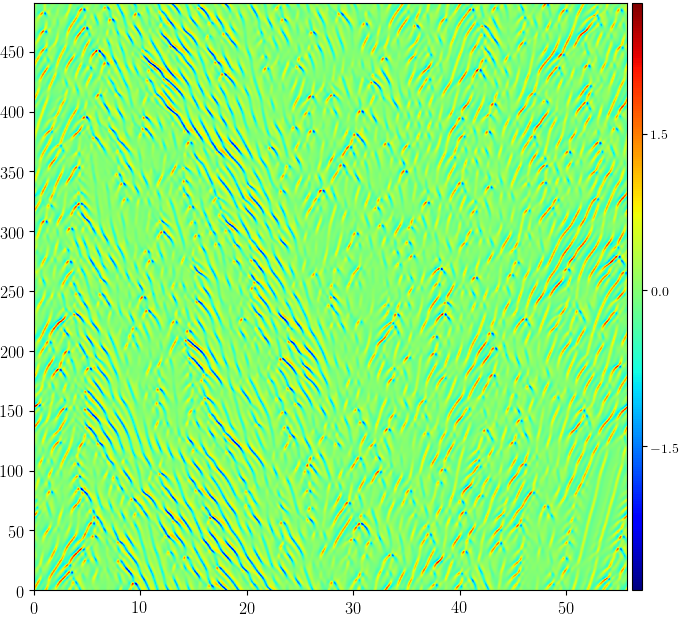
\includegraphics[width=1.0\textwidth]{MNG_ut_largeL}
%\\ \small{\texttt{(a)}}
%\end{minipage}
%\begin{minipage}[height=.48\textheight]{.48\textwidth}
%\centering \small{
%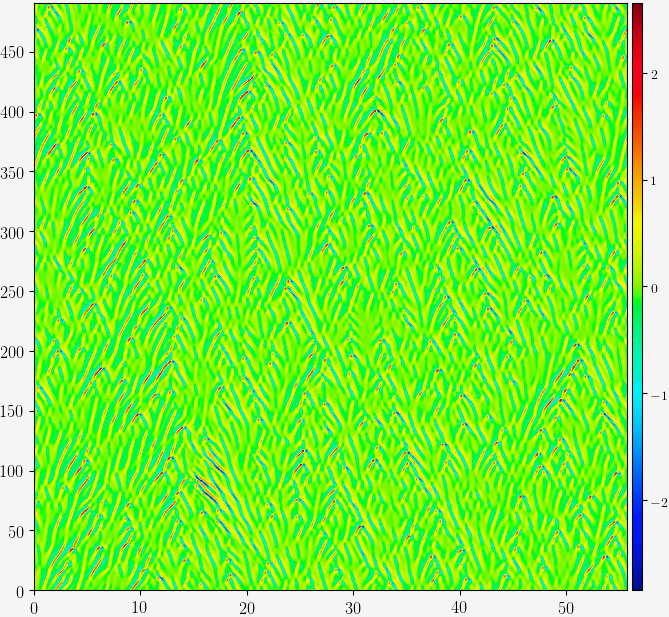
\includegraphics[width=1.0\textwidth]{MNG_ut_largeL2000}
%\\ \texttt{(b)}}
%\end{minipage}
%\caption{\label{f:MNG_ut_largeLtrans}
%On dangers of peculiar initial conditions.
%(a)
%A transient {\spt} \KS\ solution, transient time $\period{} \approx 50$:
%the first temporal derivative $u_\zeit$.
%(b)
%A typical {\spt} ``steady state turbulent'' \KS\ solution $u_\zeit(\conf,\zeit)$,
%after a long time transient $\period{} \approx 2\,000$ exhibits no long-range
%correlations, only short left or right travelling waves, ending in collisions.
%Suggests a nice 3 letter alphabet.
%The first temporal derivative
%$u_\zeit = -u\,u_\conf - u_{\conf \conf} - u_{\conf \conf \conf \conf}$
%is a Galilean invariant field. The figure color is manipulated to emphasize
%the pattern.
%     }
%\end{figure}
%%%%%%%%%%%%%%%%%%%%%%%%%%%%%%%%%%%%%%%%%%%%%%%%%%%%%%%%%%%%%%%%%%

\MNGpost{2019-05-13}{
Let me preface the discussion with saying that the colorbar units
(displaying the range $[-1.5,1.5]$) is an adopted convention for
\twot\ figures
so that all velocity fields are displayed on the same scale.
Generically, if one integrates the \KSe\ defined on a domain
with small $\speriod{}$ (\ie\ the size of tiles) then the average for
the local minima and maxima over a large number of trials is
$\approx 2.6$. The minima and maxima for the tiles are as follows
\\

\begin{tabular}{c|c|c}
                & maxima & minima \\
\text{defect \#1}& 2.53 & -2.64 \\
\text{defect \#2}& 2.00 & -2.37 \\
\text{hook}& 2.40 & -2.67 \\
\text{gap}& 2.49 & -2.47 \\
\text{streak}& 1.21 & -1.21
\end{tabular}
\\

upon further inspection the values for
the solutions seem to match the time
integrated simulations but the value
for the streak is worrisome until one,
once again, performs numerical simulations
on a domain size comparable to that of the streak
domain $\speriod{} \approx 6.39,
\frac{L}{2\pi}\approx 1$. So in summary the values of the colorbar
as exaggerated by the convention to fix the
limits of the colorbar. This convention was
not employed for \reffig{f:MNG_largeLtrans}, which
is predominately the reason for the discrepancy.

As to \emph{why} the value of local maxima(minima)
increase(decrease) as a function of L, I don't have
a better argument than the extensive nature of the \KSe.
It is sometimes useful to modify the magnitude of $u$
when gluing, which can probably be explained by approaching
the upper bound of $u$ from above is numerically
beneficial. For instance, I would never use
streaks bounded between values exhibited by \reffig{fig:MNGtiles}, but the
solution exists with those bounds at that domain size regardless.
Therefore, to take the extensive property of the \KSe\ into account
it is fairly common to rescale the tiles from \reffig{fig:MNGtiles}
to suit the situation and better fit together. This
is not equivalent to using Galilean symmetry group orbit
as the rescaled solutions still satisfy the mean velocity condition.

I agree that the mean velocity constraint is not satisfied locally ;
this was the basis behind my idea of ``stabilizing'' spatial integration
by somehow incorporating a ``local'' Galilean symmetry but I never figured
out how to do it or even what I really meant by this.

Incorporating the degree of freedom provided by the Galilean invariance
would likely make finding solutions easier (in a least squares sense)
because it increases the codimension of the group orbit of solutions, identically
to translations (I don't do any slicing or use Poincar\'e sections for this exact reason;
why impose such strict constraints when there is no reason to a the moment?).
I never really thought of this, as it is another case of being too comfortable
with the conventions developed for time dynamical systems.
I'll try to work through this idea but it would be a pretty sizeable upheaval as
most of my code eliminates the zeroth spatial modes; something that can
be shelved for later.
}

\PCpost{2019-05-14}{
Looking at \reffig{f:MNG_ux_largeLtrans} and \reffig{f:MNG_ut_largeLtrans}: we might
chose Galilean invariant elementary tiles (spatial derivatives of $u$),
instead of Galilean equivariant $u_j$ tiles of \reffig{fig:MNGtiles}.
}

\PCpost{2019-05-14}{
Which brings me back to \reffig{fig:MNG_spacetime_capped}\,(b).
Can you start with a \reffig{fig:MNG_spacetime_smoothed} smoothed and
$\bar{L}=2\pi\sqrt{2}$ modulated ``noise'' initial guess on
$(\speriod{},\period{})=(500,500)$, run it through your optimizer - do
you get a small error, and something that looks like
$(u,u_\zeit,u_\conf)$  of \reffig{f:MNG_largeLtrans}?
Maybe the answer is already your \reffig{fig:MNGlarge_adjointdescent},
but that looks nothing like \reffig{f:MNG_largeLtrans},
so it worries me.

We need such figures
anyway to illustrate your initial guesses.
}

\MNGpost{2019-05-16}{
Trying to see if I can get a nice large-domain adjoint descent
optimization; its been a while since I tried. I spent some time tweaking
my codes to try and get the best results but this still needs a bit of
work. Not investing too much time in this, I think I just need a large
chunk of computation time and something decent should pop out.

Results from large domains like \reffig{f:MNG_largeLtrans} when
starting with modulated noise are hard and I never really gave it much
effort because of its likelihood to work and or priority not to mention
the amount of time it takes. I'm attempting some trials now so hopefully
I will have something that looks  better than \reffig{fig:MNGlarge_adjointdescent}
in the near future.
}

\PCpost{2019-05-15}{ Plumbers' hangout:
Predrag showed Matt's latest plots of \KS\ velocity field
$u$, its spatial gradient $u_x$ and its time derivative $u_t$ on a large
$(\speriod{},\period{})=(500,500)$ spacetime domain (that is $\approx 55$
wiggles of $u$ across $x$-axis), \reffig{f:MNG_largeLtrans}. The most striking
is the $u_t$ plot - clearly visible is a dominant $\pm$ {\phaseVel} which
implies there are long range correlations, in time at least as long as
the entire pattern of time period
$\period{}=500$.
\\
{\bf 2019-05-20 Predrag} \reffig{f:MNG_largeLtrans}\,(a) is a lesson
in dangers of using strange initial conditions, not checking whether transients
have died out. As illustrated by \reffig{f:MNG_largeLtrans}\,(b), there are
weird `letters', no long range correlations.

This violates our common intuition that \KS\ decorrelates exponentially
both in space and time. Burak showed us (again) the earliest simulation
of turbulent body-forced 3D cube (again Predrag forgets the authors)
which shows very clearly that the turbulent flow has long correlations in
form of long vortex tubes. That does not help with 1D \KS\ - no vortex
tubes...
}

\PCpost{2019-05-15}{
Which brings me back to \reffig{fig:MNG_spacetime_capped}\,(b). We
usually plot \refeq{EnRate} which balances the power $P$ pumped in by
anti-diffusion $u_{xx}$ against the energy dissipation rate $D$ by
hyper-viscosity $u_{xxxx}$ in the \KSe.  So it might be nice to have look
at plots of local power $\half u_{x}^2$, dissipation $\half u_{xx}^2$,
and energy rate (the difference of the two).

All of the above were derived by thinking ``in time''. Might have to
rethink all of these in spacetime. In particular, might plot the 4\dmn\
vector field \refeq{e-ksX} as well.
}

%\begin{figure} %[t]
%\begin{minipage}[height=.5\textheight]{.5\textwidth}
%\centering
%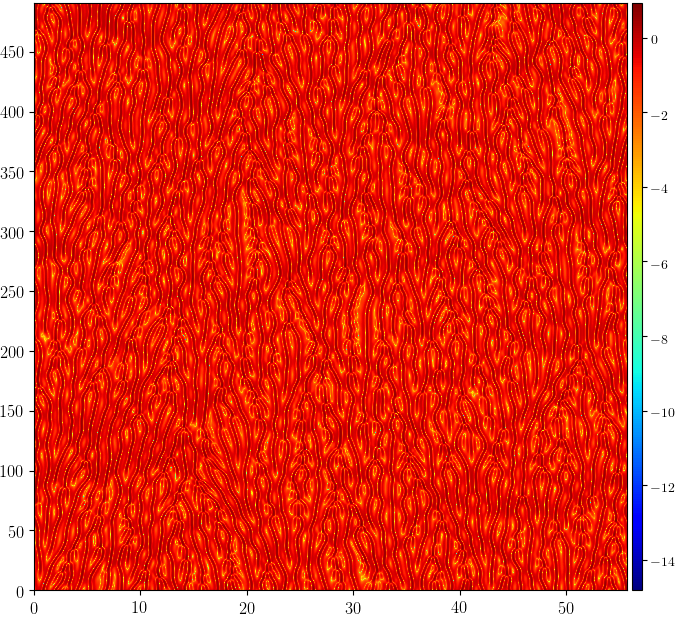
\includegraphics[width=1.0\textwidth]{MNG_P_largeL2000} %what is {MNG_P_largeL}?
%\\ \small{\texttt{(a)}}
%\end{minipage}
%~~~~
%\begin{minipage}[height=.27\textheight]{.27\textwidth}
%\centering
%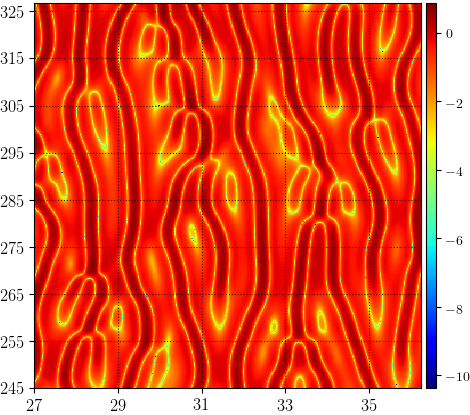
\includegraphics[width=1.0\textwidth]{MNG_P_largeLsub2000} %what is {MNG_P_largeLsub}?
%\\ \small{\texttt{(b)}}
%\end{minipage}
%\caption{\label{f:MNGPlargeL}
%(a)
%Power density $\half u_{x}(\conf,\zeit)^2$ of the {\spt}
%``steady state turbulent'' solution, \reffig{f:MNG_largeLtrans}\,(b).
%(b)
%A zoom into a subdomain of (a), spatial width $\speriod{}=54 \approx 6.17
%\times 2\pi\sqrt{2}$.
%Power density exhibits a maximum in the region between every
%``wavelength'' (maximum minimum pair): in order to go from local maximum
%to local minimum on the shortest length scale the first derivative must
%take on near maximal values to account for the rate of change of
%$u(\conf,\zeit)$.
%     }
%\end{figure}
%
%\begin{figure}[t]
%\begin{minipage}[height=.5\textheight]{.5\textwidth}
%\centering
%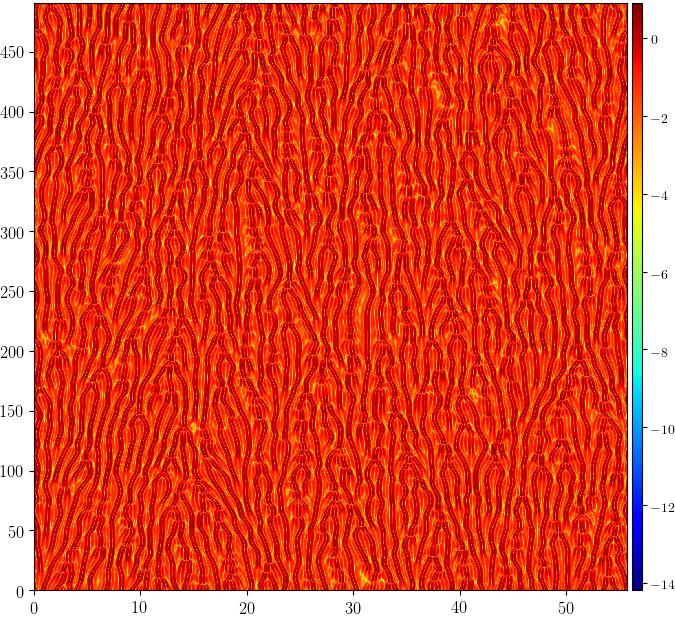
\includegraphics[width=1.0\textwidth]{MNG_D_largeL}
%\\ \small{\texttt{(a)}}
%\end{minipage}
%~~~~
%\begin{minipage}[height=.27\textheight]{.27\textwidth}
%\centering
%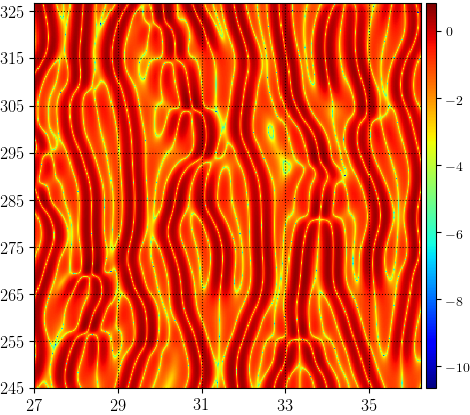
\includegraphics[width=1.0\textwidth]{MNG_D_largeLsub}
%\\ \small{\texttt{(b)}}
%\end{minipage}
%\caption{\label{f:MNGDlargeL}
%(a)
%The dissipation rate density $\half u_{xx}(\conf,\zeit)^2$ of the {\spt}
%solution of \reffig{f:MNG_largeLtrans}\,(b).
%(b)
%The subdomain of \reffig{f:MNGPlargeL}\,(b). The dissipation rate
%density is maximized at the maxima and minima of $u(\conf,\zeit)$ because
%these are the values when the second spatial derivative is largest.
%Around two-to-one wavelength mergers or ``defects'' (e.g. around
%coordinates (9,75), (12,95)) there is a dramatic increase in the
%dissipation rate, similar to the power density \reffig{f:MNGPlargeL}.
%     }
%\end{figure}
%
%\begin{figure}[t]
%\begin{minipage}[height=.5\textheight]{.5\textwidth}
%\centering
%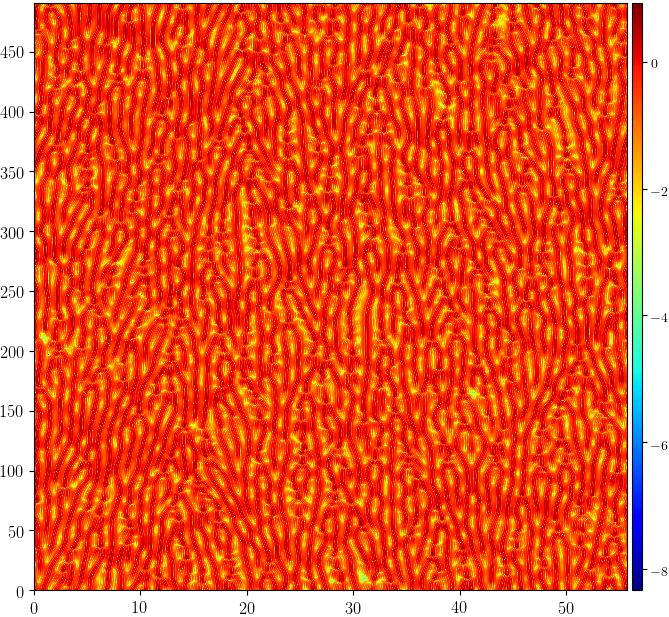
\includegraphics[width=1.0\textwidth]{MNG_E_largeL}\\
%\small{\texttt{(a)}}
%\end{minipage}
%~~~~
%\begin{minipage}[height=.27\textheight]{.27\textwidth}
%\centering
%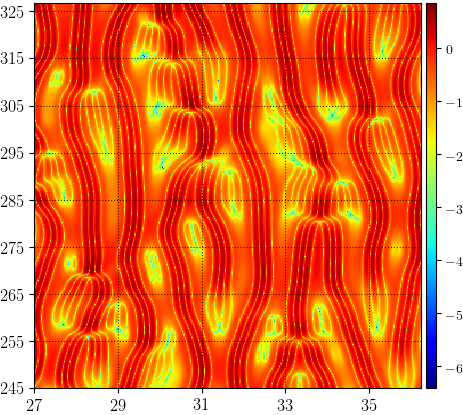
\includegraphics[width=1.0\textwidth]{MNG_E_largeLsub}\\
%\small{\texttt{(b)}}
%\end{minipage}
%\caption{\label{f:MNGElargeL}
%(a)
%The local energy density rate $\half u_{x}^2 -\half u_{xx}^2$ of the {\spt}
%solution of \reffig{f:MNG_largeLtrans}\,(b).
%(b)
%The subdomain of \reffig{f:MNGPlargeL}\,(b).
%Due to the dependence on the power and dissipation we can
%see that the energy rate is maximized near the same regions as
%the power and dissipation. The power maxima sit on nodes of each
%wavelength while the dissipation maxima are located at the crest and
%trough of each wavelength. This phase difference ensures that the local
%energy rate is non-zero.
%There are two typical patterns for regions of maximal
%energy rate. The highly localized defects
%at $\approx(9,75)$ and $\approx(12,95)$ and much
%broader patterns like the region from $t \in [114,134],
%\forall x$.
%     }
%\end{figure}

\begin{figure}[t]
\begin{minipage}[height=.30\textheight]{.30\textwidth}
\centering
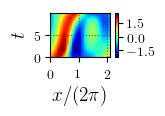
\includegraphics[width=1.0\textwidth]{rpo_L13p08_T9}
\\ \small{\texttt{(a)}}
\end{minipage}
\begin{minipage}[height=.30\textheight]{.30\textwidth}
\centering
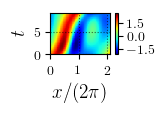
\includegraphics[width=1.0\textwidth]{rpo_L13p09_T9}
\\ \small{\texttt{(b)}}
\end{minipage}
\begin{minipage}[height=.30\textheight]{.30\textwidth}
\centering \small{
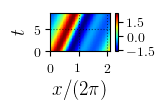
\includegraphics[width=1.0\textwidth]{rpo_L13p10_T8}
\\ \texttt{(c)}}
\end{minipage}
\caption{\label{f:MNGhookshedding}
Members of the continuous family of defects (2-to-1 wavelength mergers)
numerically continued and converged at spatial domain sizes
(a) $\speriod{}=13.08$, (b) $\speriod{}=13.09$, (c) $\speriod{}=13.10$.
%(these are exact, due to continuation constraints).
Here not stated in ``natural'' units of $2\pi \sqrt{2}$ because of their
proximity.
(a)
Is most reminiscent of the defect family,
specifically the pattern previously often called the ``hook''.
(b)
As the ``hook'' gains an increasing \reqv\ \spt\ shift it ``tilts'' more and
more until it finally bifurcates into
a \reqv\ solution (c).
The ``hook shedding'' mentioned (somewhere?) in sits precariously between (b) and (c).
}
\end{figure}

\MNGpost{2019-05-16}{
Produced \reffig{f:MNGPlargeL}, \reffig{f:MNGDlargeL},
\reffig{f:MNGElargeL}, which are the power, dissipation and energy
density rates respectively for the large \spt\ data set
\reffig{f:MNG_largeLtrans}\,(b), \PCedit{plotted on a logarithmic scale
and thus looking like red lobsters}. These look like to me like many
different things, white caps in the ocean, a fan, a dispersing wave, a
beat-like pattern.
    \PC{2019-05-20}{
    why all duplicate figures \texttt{MNG\_P\_largeL2000.png} =
    \texttt{MNG\_P\_largeL.png}, \etc?
    }

The energy rate seems to display two main
behaviors, a highly localized maxima at 2 to 1 wavelength
defects and then a much broader pattern of increased
energy rate in the shape of a fan, patch, beat, wave
or any other shape left to one's imagination.
}

\MNGpost{2019-05-16}{
Regarding above comments on \reffig{f:MNG_largeLtrans}\,(a):

$u_\zeit = -u\,u_\conf - u_{\conf \conf} - u_{\conf \conf \conf \conf}$
is a Galilean invariant field. There is a very prominent leftward /
rightward wave propagation speed, perhaps several. But the result is
puzzling: on the left half, there are prominent leftward moving reddish
lines - but there are no prominent rightward moving bluish lines. Also,
both figures reveal a very persistent structure (not in our alphabet?)
from $(\conf,\zeit) = (9,0)$ to $(10,130)$ with a smaller wave velocity
(note, the \conf-axis is mislabelled).

In regards to this ``missing letter'', I have an explanation (as Senator
Warren says, I have a plan for that) but its a very specific case of a
known ``letter'' so I had not mentioned before. The reason for the lack
of inclusion of the coherent \reqva\ structure in the bottom right hand
corner of \reffig{f:MNG_largeLtrans}\,(a) is because it sits right at the ``edge''
of the defect family before it transitions into a \reqv\ solution.
This phenomenon occurs around $\speriod{}\approx 1.47\times 2\pi\sqrt{2}$.
}

\MNGpost{2019-05-16}{
Viewed as a decreasing function of $\speriod{}$, the \reqv\ undergoes a
bifurcation (I haven't inspected any eigenvalues), likely a Hopf bifurcation,
such that there is an additional (quasi) periodic behavior which is very coarsely
analogous to ``vortex shedding'', except in this case its ``hook shedding'' as a
function of time. The likely reason behind its presumed quasi-periodicity
exhibited in \reffig{f:MNG_largeLtrans}\,(a) is due to local \spt\ coupling. I surmise that
the bottom right hand corner of \reffig{f:MNG_largeLtrans}\,(a) consists (perhaps
surprisingly) of members of the same defect family which pervades the entire
plot.

Three `rubber tiles' in this family which display this phenomenon are shown in
\reffig{f:MNGhookshedding}.
Note: old figs, so old units.
}

\MNGpost{2019-05-16}{
Correction: the above ``missing letter'' seems to have been artifact of my
time-froward integrations staring with a suspiciously symmetric initial
condition. Now that I've increased transient time from $\period{} \approx 50$ to
$\period{} \approx 2,000$, all weird things, including the ``missing letter,''
are gone.
}

\PCpost{2019-05-16}{
Keep the short-initial-transient \texttt{*.png}'s in figures
\ref{f:MNG_largeLtrans}\,(a)-\ref{f:MNG_ut_largeLtrans}\,(b)
under current file names.
Give slightly different names to your asymptotic \texttt{*.png}'s, transient time
$\period{} \approx 2,000$ . The pre-asymptotic figures are educational for us,
internally, keep them.
}

\MNGpost{2019-05-19}{
\begin{description}
\item[Takashi Tokieda]
Chain fountain (Newton's beads) demonstration. Theorem from the 19th century
Once it gets going, a chain can flow in any shape in neutral equilibrium.

Looking at the net forces of a infinitesimal section of  the chain.
By the normal component of tension, if the flow
is fast enough then the tension is independent of the
radius of curvature (geometry becomes irrelevant).

This is an anomalous reaction, which appears to violate Newton's third law.
A toy model for this phenomenon is a free-falling rod which lands
at an angle to the ground, such that one end hits first. This contact
with the ground induces a torque which ``pulls'' the end of the rod
down faster.
(Movie by Andy Ruina) of rope ladders falling, one that makes contact
ends up falling faster. This is an example of tension resulting
from compression. This model relies on the
bending stiffness of the rods.

(Very) Basic model for the rod example using Newtonian mechanics,
Half of the energy is lost to the shock dissipation.

Using this, estimate how high the newton's beads should go.
Zigzag monolayer has only horizontal components, yet there
is a vertical arching. Criticality (where derivative vanishes)
is taken advantage of the change.

Why does the chain stand up vertically?
Very singular phenomenon of minimum chain radius. Curvature induced
at the location of horizontal motion. The accumulated curvatures
of the curl induce buckling due to torsion.

WHITE PINE

\item[Qiqi Wang]
\textbf{Computation of sensitivities in chaotic systems: an overview}
Overview of sensitivities in chaotic simulations.

Going to use a very real example. Using the
buffets of F35 (raptor?). Shaking is
due to vortex breakdown (chaos). Chaotic
aerodynamics cause aircraft buffet.
This also takes place with (space)
launch vehicles. Length makes it
so most of the body is actually in the wake of
the front end. Yet another example: chaotic
aerodynamics melts engine components.
This mini symposium is dedicated to
sensitivity analysis and optimization
of chaotic dynamical systems, not merely
simulation.

How is the objective function (structural
damage, long time average heat transfer).

steps
\begin{enumerate}
\item Parameterize the autonomous equations
\item Define the objective function (average quantities,
instantaneous quantities not really defined).
\item Compute the derivative of the objective function
with respect to the parameters.
\end{enumerate}

Why not use finite difference for sensitivity of statistics?
Extremely inefficient. Argument:
let X be a random variable in a uniform probability
distribution on $[0,s]$. The derivative of the mean
is equal to half. Sampling error (finite difference
implies cancellation error?) ruins the
finite difference scheme, this error is amplified
by dividing by ds.
Error decreases as the square root of the sample size.

Using the Lorenz equations, define the objective
function as the average of the deviation of $z$
from some mean. The ``design parameter'' is
$\rho$ from Lorenz. Looks like noise at low
sample size.

For ``small problems'' you can parameterize the
2D slice

Adjoint: differentiation the output of a simulation
to its inputs by tracing backwards through the calculations.
The problem with this is that it doesn't work because of the
instability.

Can we desensitize the adjoint method to the noise
in computed statistics of chaotic simulations.

Parameter perturbation vs initial condition perturbation.

Question: Implicitly there is some flow
which is very high dimensional, is this always with
normally this would be an incredibly
high dimensional problem, is the flow not
a variable? Is the base flow always stable?

\item[Angxiu Ni]
\textbf{Adjoint Shadowing direction in Chaotic Dynamical Systems for
sensitivity analysis}
Classical trajectory-based sensitivity analysis fails.
Small scale variations has much more profound effect on
the ``zoom in'' slope as opposed to the ``zoom out'' slope.
Zoom in, let $ds\to 0$ and then $T\to \infty$
Zoom out, let $T\to \infty$ then $ds\to 0$.
\beq
\frac{Javg}{} = \frac{d}{ds} \lim_{t\to \inf}
\frac{1}{t} \int \partial_u J \frac{du}{ds} + \partial_s J dt
\eeq
Shadowing lemma: two kinds of perturbations. Perturb initial conditions, keep
parameters and vice versa. If you do both, and they are coordinated, can
remain close ($L_2$ norm of perpendicular distance (pointwise?)). Is this
always continuous? bifurcations?

Changing the initial condition uses covariant Lyapunov vectors (homogeneous
tangent equation). Changing the parameters results in inhomogeneous tangent
equations.

\beq
\frac{J_avg}{ds} \approx !/T \int_0^T [|partial_u f v^{\perp} +\partial_s J + \eta (J-<J>)
\eeq
Interpretation of terms, in order,
state space ``location difference'', direct dependence of J on s and the speed difference term.

This was tangent space definition, now onto the Adjoint shadowing direction now.
\beq \frac{d<J>}{ds} = 1/T <v,J_u>_{L_2} \eeq
\beq v(t) = \frac{\delta u}{\delta s} \eeq

Propagate stable parts forward, unstable part backwards. ``Dual'' derivation.
Let
\beq \bar{v}(t) = T\frac{\delta <J>}{\delta u(t)}\eeq

Conditions of $\bar{v}$ imply adjoint shadowing direction, approximation of
real adjoint shadowing direction.
\beq \frac{dJ_{\infty}}{ds}\approx 1/T<\partial_s f, \bar{v}>_{L_2} \eeq

\textit{Non-Intrusive Least-Squares Adjoint Shadowing}
Adjoint flow and tangent flow have similar structures, which allows for
recycling of least squares shadowing ideas.

Violates the adjoint shadowing lemma but still works fine?
Can't prove but still works well in practice. It still
works as long as unstable directions are not orthogonal?

\item[Nisha Chandramoorthy]
\textbf{Space-split statistical sensitivity computation
in chaotic systems}
Autonomous equations, forward time mapping, time discretized
PDE or forward time mapping.

Split tangent space into stable and unstable manifolds. Unique
ergodic invariant physical measure (SRB). Work with
uniform hyperbolic chaotic systems. Cat map example.


PRIMROSE A
\item[Chris Marcotte]
\textbf{Sensitivity of spiral wave core formation
 and transient spiral core interactions}
Very behind schedule or is this dude taking all of Chris' time?
Adjoint eigenfunctions and singular modes are the subject of his
talk. Cardiac rhythms and arrhythmia.
Using very simplified excitable models. Model allows for
sustained spiral chaos. Spiral cores born in pairs die
in pairs. Tangent space flow via linearization, and
its adjoint

Tangent flow modes are global while adjoint modes are localized.
Can quantify this localization. Adjoint modes tell us how perturbations
generate transitions. Floquets modes (tangent space eigenmodes)
characterize stability of solutions.

Open trajectory, when linearization fails due to distance of successive
points on the trajectory. Using Golub, Kahan (probably based on Ginelli).
Display of singular modes with respect to time.

\item[Andrew Krause]
\textbf{Pattern formation in bulk-surface
reaction diffusion systems}

Turing instabilities and chemical morphogenesis
(how you see symmetry breaking in-vivo).
Have two reaction-diffusion equations which are
coupled. Mouse whiskers develop sequentially.
Microsoft is genetically engineering bacteria.
Develop in-vivo Turing patterns and instabilities.

Classical dispersion relation and stability
analysis

Linearize autonomous system around spatially steady state
and use (Lindstedt) ansatz which is base flow plus
exponential growth term.

Instabilities on spheres and tori. Influence of
curvature, growth, anisotropy. Laplacian
is space dependent but can solve via spectral problem.


\beq det(M_k) = \text{det}(\lambda_k - \rho_k D_k - J_k)
\eeq

Multiregion domains
Super complicated, cannot reduce problem via
symmetry arguments so have to work
on full problem. Cannot solve eigenvalue
problem as a function of depth ($y$)
due to coupling. Try anyway,
get solutions and some expression
for determinant and hence the dispersion relation.
Nontrivial coupling, relating heterogeneity
to some strength parameter.

Turing instabilities in heterogeneous domains.
In reaction kinetics (not the transport)
is heterogeneous. Other than the initial
bifurcation (one to two cells), every pattern
does not occur on homogeneous background. Mouse
and chicken modeling, simulations capture some
behavior. Linear analysis on heterogeneous domains
via WKB ansatz. WKB modes are not supported on
same domains.

\item[Raquel Gonzalez Farina]
\textbf{Dynamics from a coupled chemical thermal
microsilica partical formation model}

Information of chemical reaction.
Microsilica particles are spherical and growth
is mediated by nucleation,condensation and aggregation (combining)
Want to control the furnace to control the properties of the
microsilica.

\textbf{Initially well mixed chemical species}
One dimensional geometry, conservation equations
for all chemicals,temperature and number density of particles.

Uniform concentrations, no diffusion terms. Boundary
conditions on flux is related to particle number and
nucleation rate, otherwise straightforward.

Derivation of dimensionless quantities and various
growth and nucleation rates.

Analytical solution when $\zeta_i=0$ (nonlinear
coupling constants). Can then solve for an
analytical solution of the particle
density equation (method of characteristics).
Divergent particle side.

Now set $\zeta_i\neq 0$. Something about
equations being coupled except with respect
to one degree of freedom? Asymptotic particle size.

\textbf{Spatially heterogeneous chemical concentrations}
Diffusion
comes back into the equations. Proof that there are
no \reqva\ but can find solutions that have some
properties of \reqva\ and self-similar solutions.

Diffusion dominant for small times and reactions
dominant are large times? (obvious?, concentration
approaches steady state no?)

Coupling makes it so particle size distribution
pushes small particles into the ``middle''.

Future: more realistic flow and furnace geometry.

\item[Robert Van Gorder]
\textbf{Pattern Formation in reaction-diffusion systems
 on time-evolving domains}
Loss of stability of spatially homogeneous steady states for
such systems can signal the onset of pattern formation.

Turing instabilities on state domains, the conditions
for the onset of instability are algebraic. This
is not the case for growing domains. Evolving
is not the same as growing. Turing conditions for
time-evolving domains. Want a linearly stable
steady state in order to get a Turing instability.
This leads to complex exponential solutions, conditions
on the determinant for inducing a Turing instability.
This extends to arbitrary manifolds, as long
as spectrum and eigenvectors can be determined.

Manifold now depends on time now. Simple case
of dilation as the ``equations of motion'' for
the manifold. Transform to co-moving coordinates.
Spatial dependence when other evolution types
are considered. In this case only time dependence.
Steady state was perturbed spatially, but
now the underlying state is dependent on
time (this is a choice which makes the problem harder).
Derive the linearized problem. Cannot rely
on eigenvalues and eigenfunctions due to
time dependence. Can prove linear
instability if a differential inequality
holds. Time oscillatory example was more interesting
of the two, if too fast then pattern is destroyed
(decoherence?).

Evolution of an area conserving rectangle,
volume conserving cylinder. Slow
evolution leads to spatial homogeneity
as oppose to fast evolution, where it is
still somewhat organized but less homogeneous.

\item[Piyush Grover]
\textbf{Understanding and designing emergent behavior
via stability analysis of mean field games}
Talk is in regards to multi-agent systems (swarms
of drones, traffic, etc). Features that present in nature,
desirable in engineering. This has a flavor
of an AI, machine learning, etc. talk.

Continuum (PDE) abstraction of collective
agent dynamics.

Phase space distribution
\beq \rho(x,t) = 1/N \sum \delta (x-x^k(t)) \eeq
Considering the $N\to\infty $ limit, this is not
the most common formulation so its somewhat unique.

For flocking and swarming the model that is
used is a first order model with gradient
dynamics, with homogeneous population.

ODE or SDE for each agent labeled by $i$
\beq dx_i(t) = \partial_x U(x_i) dt + 1/N \sum_j (x_j-x_i) + \sigma dw_i(t)\eeq
Using a potential that is quartic plus quadratic which is proportional to
a strength of agent behavior parameter.

The noise induces a bifurcation, when its small then the individual
motion of the agents dominate, leads to nonzero mean velocity.

Finite number of agents, introduce cost functional for each agent

\beq
J = \lim 1/T \int_0^T [\beta F[X_i,x_i-1 + \frac{1}{2\sigma^2} u_i^2(t)] dt
\eeq

Mean field approximation replaces the coupling with time dependence,
which is in turn a proxy for density. Solution of the
optimization and agent dynamics problem via
Stochastic Hamiltonian-Jacobi-Bellman theory.
HJB equation leads to (Closed loop?)
Fokker-Planck which uses
``consistency'' equations such that the
HJB is coupled to the FP equation.

Expos\'e on ``closed loop stability analysis''. Linear
stability decomposes into a local and global operators,
where the local is essentially the adjoint.
Shows that zero mean solutions become stable when
the control penalty is high and the non-zero mean solutions
are never stable.
\end{description}
}

\MNGpost{2019-05-20}{
\textbf{Gluing improvements via additional BVP}
After some thought I realized that the
method I was using to produce the initial
conditions for the gluing procedure was
a terrible idea and the truncation of the
Fourier modes was much better than the use
of convex combinations and Fourier truncation.

The reason for this is that although the smoothing
of the piecewise linear functions would result in
a continuous field that would like the constituent
\twots\ together the tangent space would be terribly
wrong. I attribute the success of the gluing in spite
of this to the potency of the \spt\ numerical methods (adjoint
descent, etc.)

I will propose an improvement (whose implementation
I will reserve for after the paper is written due to
the amount of work involved).

\item[Chebyshev BVP gluing]
The method by which I believe that solutions should be
glued, or at least the initial \twots\ should be
joined is to solve a supplementary problem which
fills in a zero padded region by virtue of approximately
solving the BVP problem induced by the connection of the boundaries
of each \twot.

Specifically, because we are more concerned with the
tangent space being correct we will utilize Neumann
boundary conditions for the BVP. Because of these
boundary conditions the ``natural'' choice for the
discretization of this connecting region is to
either used finite difference methods or
Chebyshev collocation methods. The former
is rather expedient and perhaps would be better
for this additional optimization problem because
it will not result in an exact solution either way.

The reason we know that the intermediate area
cannot have a tangent space that satisfies the \KSe\
everywhere locally is because we are connecting two
\twot\ solutions. For instance, integration of the
IVP initiated at either boundary would (theoretically)
result in the \twot\ being repeated ad infinitum.

There is still indecision on my part as to the
precise method by which the problem could be solved.

The first, a fully \spt\ method, would allow for
use of the currently implemented (with modifications
to incorporate the boundary conditions) numerical
methods. The idea is to merely follow the typical
procedure except the basis would be either Fourier-Chebyshev
or Chebyshev-Fourier depending on the gluing direction.

The second (more straightforward in my mind) method
would be to apply the variational Newton descent formalism
to a Chebyshev basis with Neumann BC. This would be
easily accomplished by using a Chebyshev basis and
differentiation operator instead of the finite difference
methods. The only difference between the spatial gluing
and temporal gluing cases would then be
the tangent space equations,
namely, whether we are using \refeq{e-Fks} or \refeq{e-ksX}
in the variational Newton descent equation.

As I'm writing this I don't think the \spt\ method would
really be that difficult. The only difference from the
current \spt\ method would be to incorporate Chebyshev
transforms and modify the differential
operators to accomodate the boundary conditions.
For instance, if tackling Neumann BC
in time then for an $N$ by $M$ time by space discretization
(Fourier in space, Chebyshev in time) then the
correct form of the equation would take the spectral
coeff
Let $u_t(A)$ and $u_t(B)$ represent the first time
derivative evaluated on the ``boundary'' of each solution.
In matrix notation we have the following
...??
}

\MNGpost{2017-08-01}{
PC recommends a paper on rigorous bounds on observables in chaotic in turbulent
flows by D. Goluskin, Tobasco, Doering, showing for instance in the Lorenz system
that the energy for points with a certain bound on the $z$ coordinate is
saturated by the equilibria, and then when $z$ increases then the energy is
saturated by the shortest periodic orbit.
}

\PCpost{2018-02-24}{
{\bf Charlie Doering} writes:
The absence proper instantaneous and/or long-time-averaged a priori bounds on
solutions of the Kuramoto-Sivashinky equation in the large interval length (L)
limit has annoyed our community for decades.

Utilizing a generalization of the background method and implementing recently
developed optimization techniques, David and Giovanni (see \arXiv{1802.08240})
have now computed rigorous bounds ––– over a large but limited range of L ––– on
the time averaged energy density of solutions that behave exactly as it is widely
believed that they should behave, i.e., $<u^2> \leq L^0$. Moreover, their method
reveals the nature of maximizing/extreme solutions: they are the largest
amplitude steady solutions on the branches bifurcating from $u = 0$.

The resulting conjecture is that this precise $O(1)$ bound holds uniformly as $L$
tends to $\infty$.
}

\PCpost{2019-05-20}{
{\bf David Goluskin}
{\em Studying Dynamics using Polynomial Optimization:}
Various global properties of nonlinear ODEs and PDEs can be inferred by
constructing functions that satisfying suitable inequalities.
Greater precision can be achieved by
using computational methods of polynomial optimization to construct functions
that satisfy the suitable inequalities.
In several examples such as
the estimation of average and extreme quantities on the attractors of the
Lorenz equations and the \KSe, polynomial optimization
produces arbitrarily sharp results.
}

\PCpost{2019-05-20}{
{\bf Giovanni Fantuzzi}
{\em Convex Analysis of Maximal Transient Growth Phenomena:}
Various global properties of nonlinear ODEs and PDEs can be inferred by
constructing functions that satisfying suitable inequalities.
Greater precision can be achieved by
using computational methods of polynomial optimization to construct functions
that satisfy the suitable inequalities.
In several examples such as
the estimation of average and extreme quantities on the attractors of the
Lorenz equations and the \KSe, polynomial optimization
produces arbitrarily sharp results.
}

\MNGpost{2019-05-21}{
\begin{description}
\item[Chad Topaz]
\textbf{A topological view of collective behavior}
Persistent homology using the Vietoris-Rips complex:
this complex is the standard for data that is organized in a point
wise fashion as opposed to \KSe\ \twot\ data in scalar-field form.

I thought that most of the talk was relatively straight forward even
with my modicum of self-taught knowledge. Every talk that I see of this
flavor leaves me with the same question, how does one extract and or classify
important patterns from the topological information. I understand that
the topological Betti numbers pick out the topological invariants
of, for instance, spatial ordering of flocks and the like. The
problem I have with this research that I have is when you are trying
to compare data that have similar but not identical topology. The
best example that comes to mind is facial recognition. Topological
data analysis would be able to tell the user that faces are connected
components and perhaps that their circular structure  would be picked up by
Betti number 1 events, but I believe the model is far too reductive
to be able to tell faces apart from one another. Perhaps this is not
the point, perhaps one would merely want to be able to pick out the number of
faces in the crowd as opposed to the specific people that they belong to.
This is a contrived example but still a question that I struggle with slash
has led me astray from Topological data analysis.
\end{description}
}

%%%%%%%%%%%%%%%%%%%%%%%%%%%%%%%%%%%%%%%%%%%%%%%%%%%%%%%%%%%%%%%%%%
\begin{figure}[t]
\begin{center}
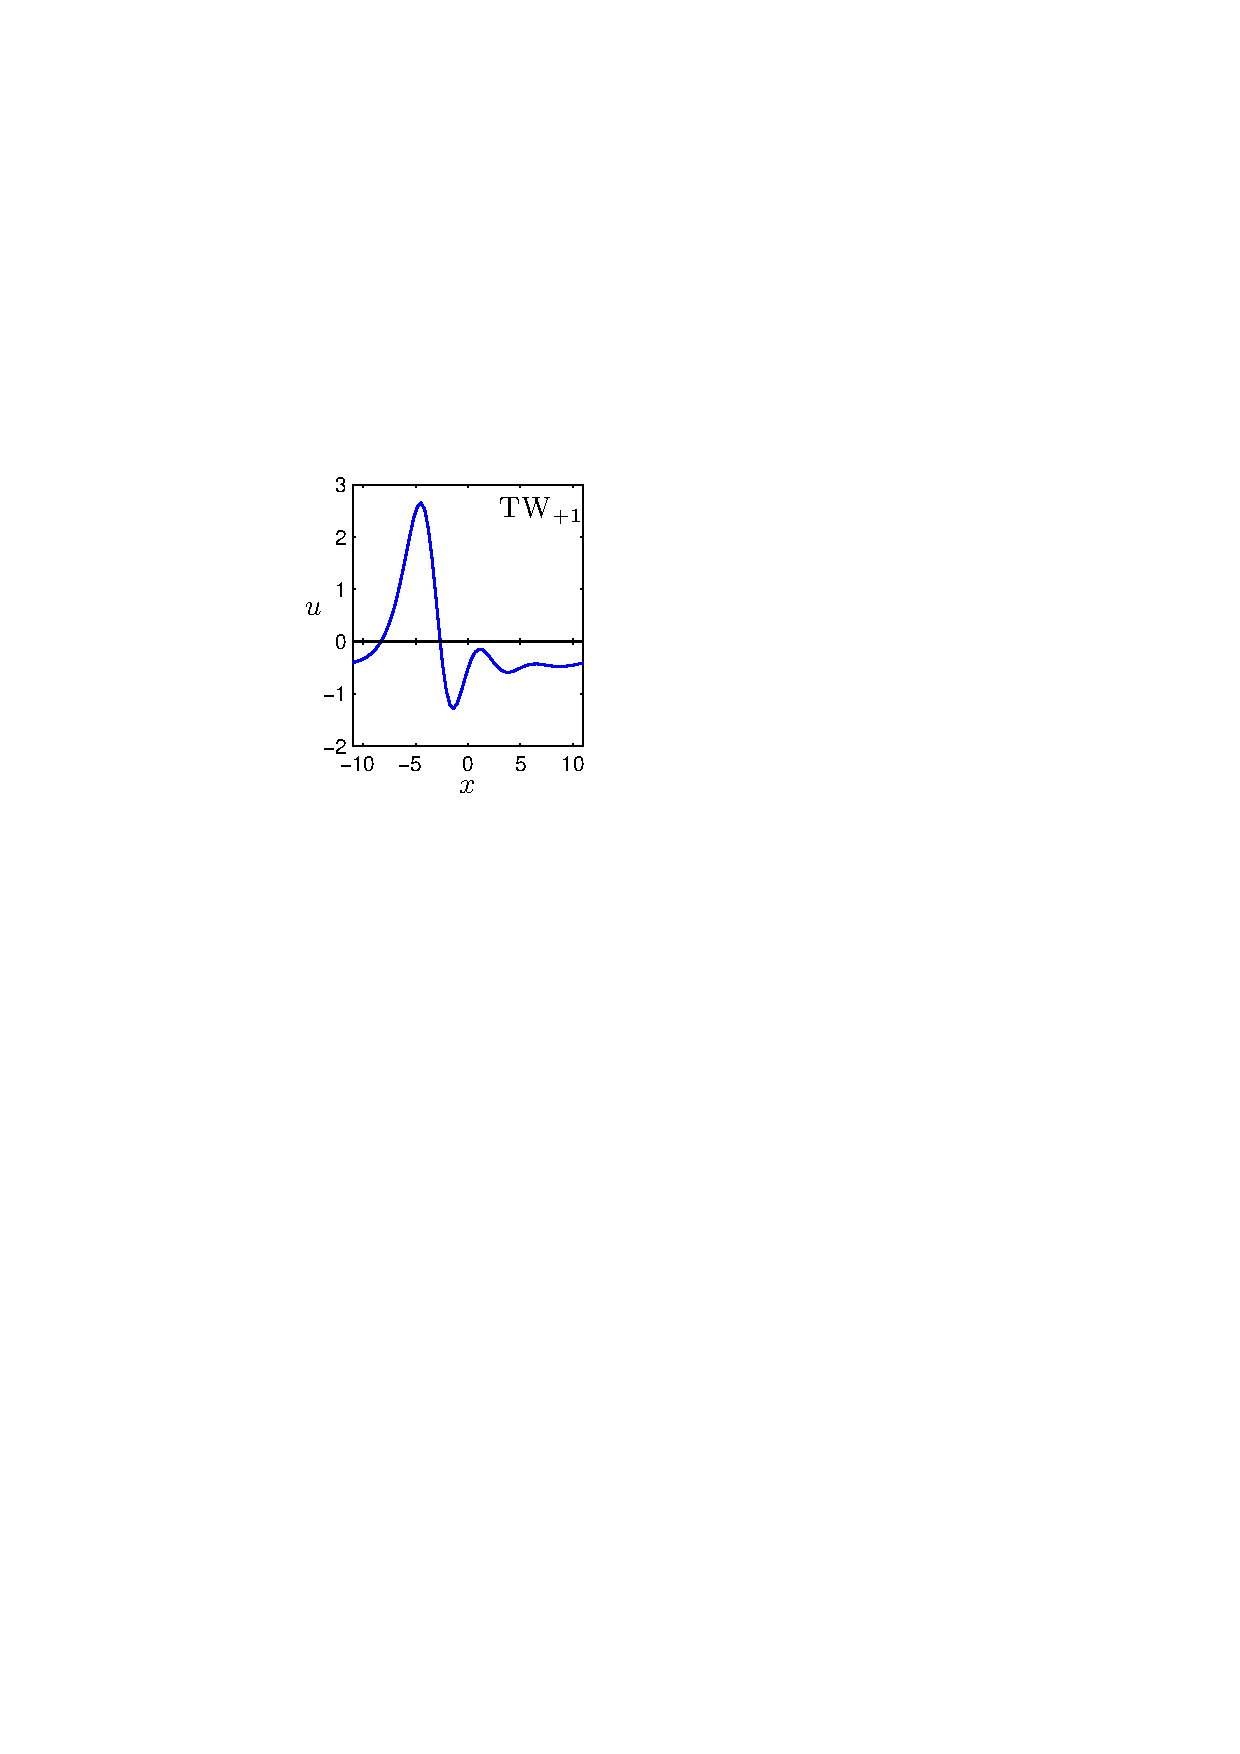
\includegraphics[width=0.3\textwidth, clip=true]{ks22_TW1_profile}
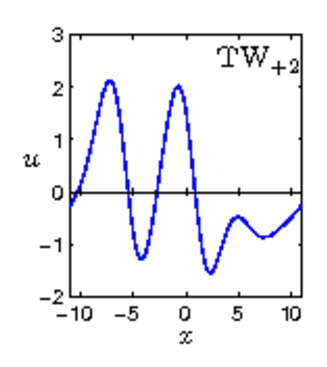
\includegraphics[width=0.3\textwidth, clip=true]{ks22_TW2_profile}\\
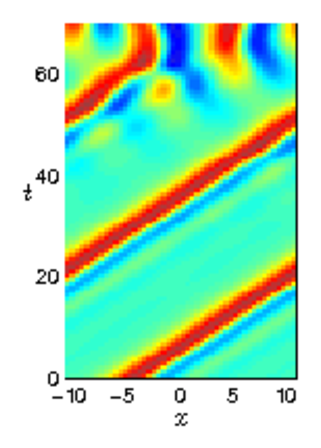
\includegraphics[width=0.3\textwidth, clip=true]{ks22_TW1_orbit_c}
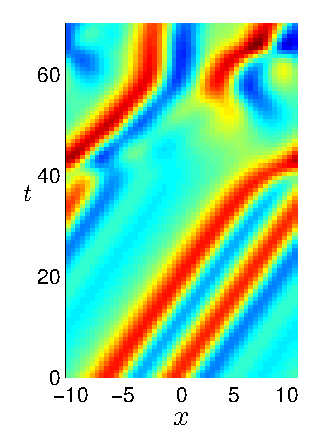
\includegraphics[width=0.3\textwidth, clip=true]{ks22_TW2_orbit_c}
\end{center}
\caption{
\Reqva : \REQV{+}{1} with velocity $c = 0.737$ and \REQV{+}{2} with
velocity $c = 0.350$.
The upper panels show the \reqva\ profiles.  The lower panels show
evolution of slightly perturbed \reqva\ and their decay into generic
turbulence. Each \reqv\ has a reflection symmetric partner related by
$u(x) \to -u(-x)$ travelling with velocity $-c$.
~~~(From \refref{SCD07}).
} \label{f:ks22TW}
\end{figure}
%%%%%%%%%%%%%%%%%%%%%%%%%%%%%%%%%%%%%%%%%%%%%%%%%%%%%%%%%%%%%%%%%%

\PCpost{2019-05-23}{
Are bits of travelling waves that dominate \reffig{f:MNG_ut_largeLtrans}?
related to either of the two \reqva\ \REQV{+}{1} and \REQV{+}{2}
of \reffig{f:ks22TW}?
}

\MNGpost{2019-05-30}{
\textbf{Matt's ultimate to-do list}
\begin{description}
\item[Short term goals]
This list contains the work that is
currently being worked on.
\begin{itemize}
\item \texttt{GuBuCv17.tex} rewrites
\item \texttt{GuBuCv17.tex} figures
\item \texttt{GuBuCv17.tex} references fleshed out
\item More thorough description of adjoint descent(garnered a lot
of attention at DS19)
\end{itemize}
\item[Intermediate term goals]
This list represents the work I would like to
complete in the next couple months.
\begin{itemize}
\item Investigate more numerical methods
\item Investigate convergence as function of $N,M$
\item Find better numerical method
for smoothing boundaries of gluing and tiling
(Chebyshev BVP, will give experience for non-periodic
boundary conditions of higher dimensional flows)
\item Investigate and improve GMRES routine
\end{itemize}

\item[Long term Goals]
This list contains the work I believe I could
finish before I graduate; I list Kolmogorov
flow because of what I have learned will dramatic
improve the efficiency with which I can code.
\begin{itemize}
\item Migrate to Julia
\item Finish papers and thesis
\item Kolmogorov with periodic boundary conditions
\end{itemize}

\item[Unicorn tier goals]
\begin{itemize}
\item Optimize Julia
\item Kolmogorov with non-periodic boundary conditions
\item Navier-Stokes with periodic boundary conditions
\item Plane-Coutte and Pipeflow
\end{itemize}
\end{description}

\textbf{Matt's GuBuCv17 to-do list}
\begin{itemize}
\item \texttt{trawl.tex} edits
\item \texttt{tile.tex} edits
\item Add continuous family description of tiles
(The misunderstandings of the tiles and how they're
used were profound and ubiquitous)
\end{itemize}

Skimmed the paper by Goluskin and Fantuzzi \rf{GolFan19}.
I need to thoroughly study the variational principles
therein but it's pretty confusing for me. Perhaps
PC and I could walk through?
Figure 1 (b) serves as corroborating evidence
for my streak tile.

The problem and or question I have is:
from a dynamical systems perspective we
know that the antisymmetric flow invariant
subspace is isolated and not representative
of the dynamics of the full (no symmetry) \KSe.
I understand that the \eqva\ exist in this
subspace so am I supposed to take this as
merely energy bounds for the antisymmetric subspace?
I feel like that defeats the point but
I don't know how else to interpret.
}

\MNGpost{07-11-2019}{
Ideas for automatic tiling using trinary tile alphabet
\begin{description}

\item[Method one]
Concatenate the scalar fields of each tile after
ensuring the discretizations accurately reflect the
relative sizes of the tiles. Fourier truncate the result.
The most basic of methods that doesn't really take anything
into consideration other than domain sizes.

\item[Method two]
The first method is to take the original
tiles and rediscretize them such that the aspect
ratios between tiles accurately represent the different
periods $T$ and domain sizes $L$ that the tiles exist on.

Put the appropriately
sized tiles (making sure the relative sizes are demonstrated
in the discretizations) together by padding them
with a boundary of zeros and then sticking the
newly sized tile plus zeros together.

This takes the sizes of the tiles and the fact that
they are discontinuous into account.

\item[Method three]
Take the existing (slightly modified and or cleaned up)
gluing code to glue the tiles together to produce one
large block of tiles that is an approximate solution.
This is then the initial condition that is passed
to the numerical methods.

\item[Method four]
The general idea is glue plus converge at every step.
This glues the tiles together in a pairwise manner just
like method three, but also takes into consideration
that the gluing combinations are only approximations
to solutions and so this goes one step further by converging
after each pairwise gluing

The quick descriptions given previously describe varying levels
of difficulty in regards to implementation
which is not necessarily indicative of improved performance.

There are a lot of important details which are so numerous
that it is actually going to take a minute to compile them all.
Currently they stand at: Making the sizes of tiles relative
to one another in a manner that still allows them to be
combined, all the while ensuring the ``best'' discretization
is being used. Dealing with the numerical discontinuity
that arises from combining tiles in space and time. Taking
into account different symmetries of tiles and the blocks
they are being used to produce.

The reason why this isn't straight forward is because
it is best to take the time to automate it as opposed
to hard coding in a case-by-case basis. As per usual
in coding, I write something only to realize that there is a
better way of doing it (rinse and repeat).
\end{description}
}

\MNGpost{2019-07-29}{
\begin{description}
\item[Symbolic Tiling code]
Running new script \texttt{blocks.py} along with
some of its new subroutines \texttt{tile.py}.

The code attempts to initialize and converge
\spt\ solutions created via combining tiles
from a trinary alphabet. The alphabet contains
the ``streak'' equilibrium solution, ``gap''
antisymmetric wave-equilibrium solution, and ``defect''
relative periodic (approximately half-cell shift solution).

The representatives chosen from each of the three
continuous families is close to being antisymmetric.
This is an intrinsic property for the gap and streak
tiles but for the defect tile, one could elect
to take the more ``hook-like'' member of the continuous
family. The hook like pattern is a member of the continuous
family which appears before numerical continuation in domain
size results in a relative equilibrium solution. The
reason for this choice is to ensure that the trinary
alphabet is symmetry invariant. This seemed the
more natural choice instead of having two
antisymmetric tiles and then a third which
has a reflection symmetry partner. That is,
a truly trinary alphabet instead of trinary plus
one symmetry partner. This might be hopeful
but its seems more elegant when the
tiles have the most in common. Numerically,
it seemed the most reasonable as the
other members of the defect family
have non-negligible spatial shift which
makes it awkward to combine with the other
tiles. In other words, it is nonsensical (to me)
to combine a relative periodic tile with a
regularly periodic tile. One of the corresponding
tiles will be non-periodic, which only depends on
whether one goes to a co-moving frame or not; again
this makes no sense in the context of combining tiles.

The automated version of the code is first searching for
combinations under the assumption that the result has no
symmetry (\ie its isotropy subgroup is the trivial subgroup).
The tiles are combined in such a manner that they are first padded
with a rectangular frame of zeros numerically, such that
zero padded tiles are arranged in a mosaic like fashion. This zero
padding is an attempt to cut down on the Gibbs' phenomenon error
associated with discontinuities.

While we know the \KSe\ is linearly unstable, and hence, including
regions of $u(x,t)=0$ is a relatively unintelligent idea, the adjoint
descent method works with such initial conditions by ``filling in''
these zero regions well. In other words, we know the adjoint descent
brings us closer to \twot\ solutions and therefore the zero
filled regions are filled in by correcting the corresponding \spt\
tangent space with local solutions such that the entire \spt\ domain
approaches a \twot\ solution. If this last paragraph was as
convoluted as I believe it might have been the general idea is
that adjoint descent brings initial conditions closer
to \twots\ by correcting the tangent space (making it abide by \KSe.)
Therefore, implementing regions with incorrect tangent space is
not an issue, so long as it does not introduce discontinuities that
make the numerical procedures fail.

\end{description}
}

%%%%%%%%%%%%%%%%%%%%%%%%%%%%%%%
%Figures included/copied from GuBuCv17 so that they can be referenced.
%

\begin{figure}
\begin{minipage}[height=.4\textheight]{.5\textwidth}
\centering
\small{\texttt{(a)}} \\
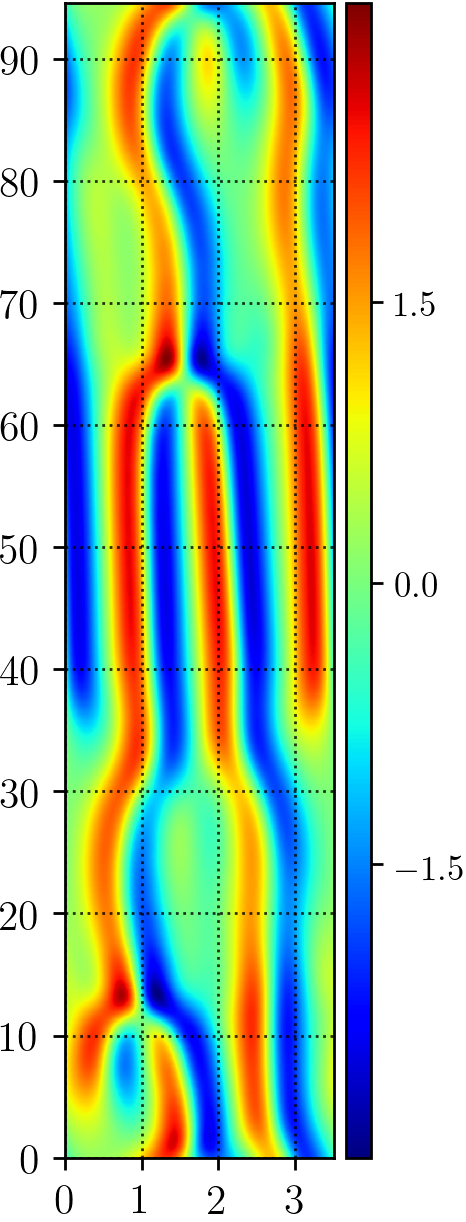
\includegraphics[width=.5\textwidth,height=.5\textheight]{MNG_halfdefect_defect_initial}
\end{minipage}
\begin{minipage}[height=.4\textheight]{.5\textwidth}
\centering
\small{\texttt{(b)}}\\
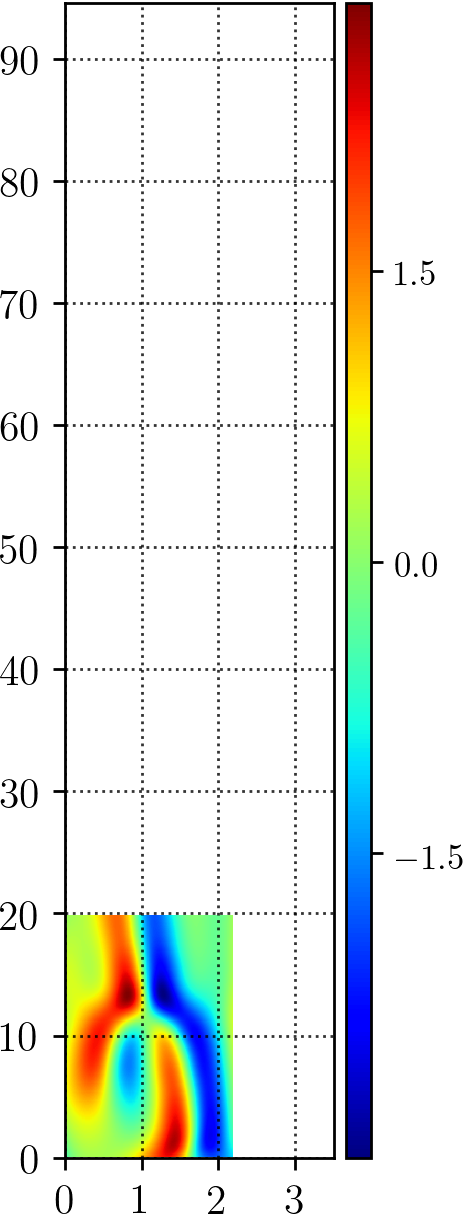
\includegraphics[width=.5\textwidth,height=.5\textheight]{MNG_halfdefect_guess}
\end{minipage}
\begin{minipage}[height=.1\textheight]{\textwidth}
\centering
\small{\texttt{(c)}}\\
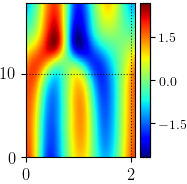
\includegraphics[width=.14\textwidth,height=.12\textheight]{MNG_halfdefect}
\end{minipage}
\caption{ \label{fig:halfdefect}
(a) \twoT\ with spatial translation symmetry defined on approximate domain $x \in [0,\approx 3.5(2\pi)]$, $t \in [0, \approx 94.59]$.  Truncation of significant digits is denoted by ``$\approx$'' .
(b) The extracted subdomain to serve as an
initial condition for tile searching. Defined on domain size $x \in [0,2.2(2\pi)]$, $t \in [0, 20]$.
}
\end{figure}

\begin{figure}
\begin{minipage}[height=.4\textheight]{.5\textwidth}
\centering
\small{\texttt{(a)}} \\
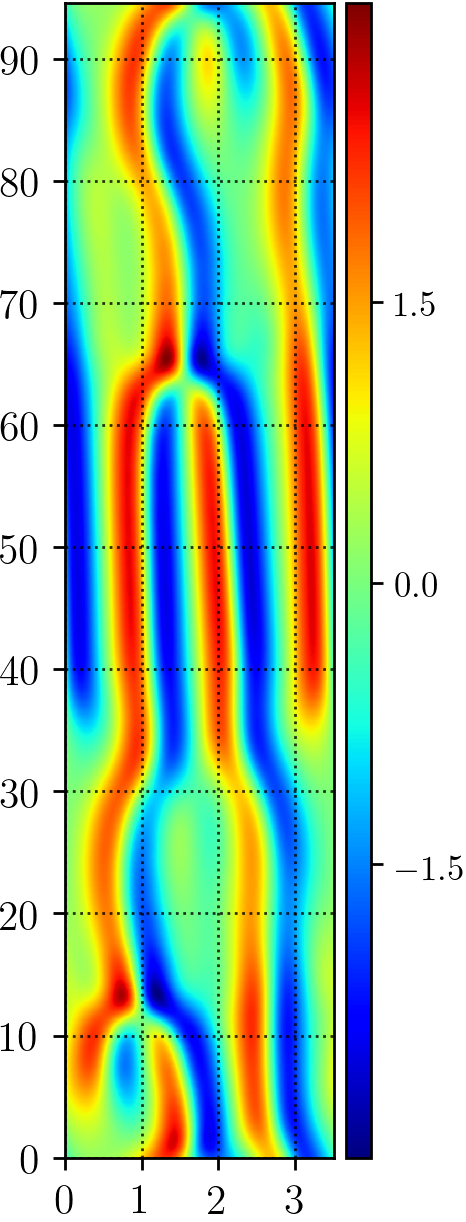
\includegraphics[width=.5\textwidth,height=.5\textheight]{MNG_halfdefect_defect_initial}
\end{minipage}
\begin{minipage}[height=.4\textheight]{.5\textwidth}
\centering
\small{\texttt{(b)}} \\
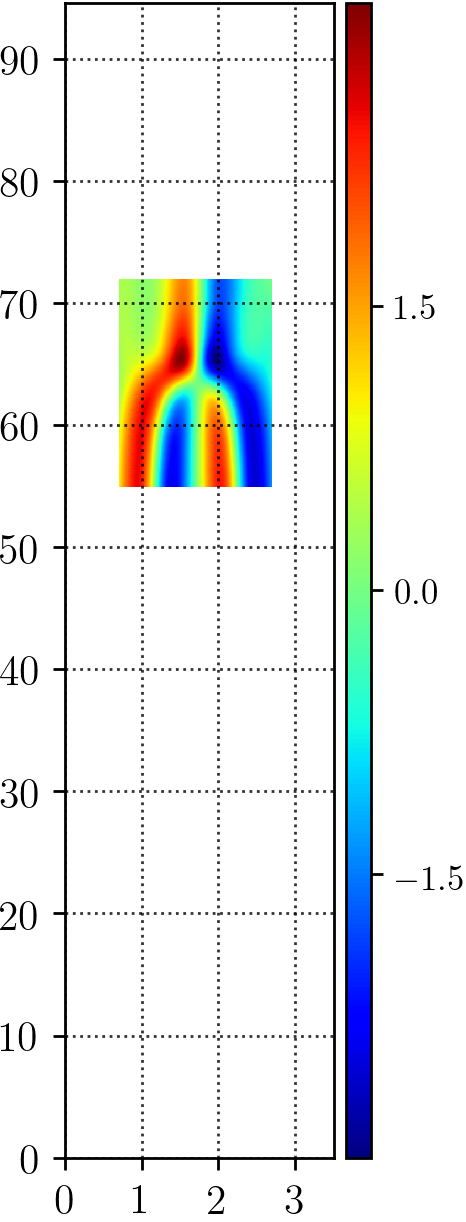
\includegraphics[width=.5\textwidth,height=.5\textheight]{MNG_defect_guess}
\end{minipage}
\begin{minipage}[height=.1\textheight]{\textwidth}
\centering
\small{\texttt{(c)}}\\
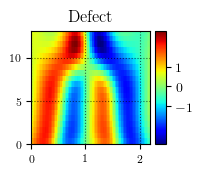
\includegraphics[width=.14\textwidth,height=.1\textheight]{MNG_defect}
\end{minipage}
\caption{ \label{fig:defect}
(a) \twoT\ with spatial translation symmetry defined on approximate domain $x \in [0,\approx 3.5(2\pi)]$, $t \in [0, \approx 94.59]$. Truncation of significant digits is denoted by ``$\approx$'' .
(b) The extracted subdomain to serve as an
initial condition for tile searching. Defined on domain size $x \in [0,2(2\pi)]$, $t \in [0, 17]$.
}
\end{figure}

\begin{figure}
\begin{minipage}[height=.4\textheight]{.5\textwidth}
\centering
\small{\texttt{(a)}} \\
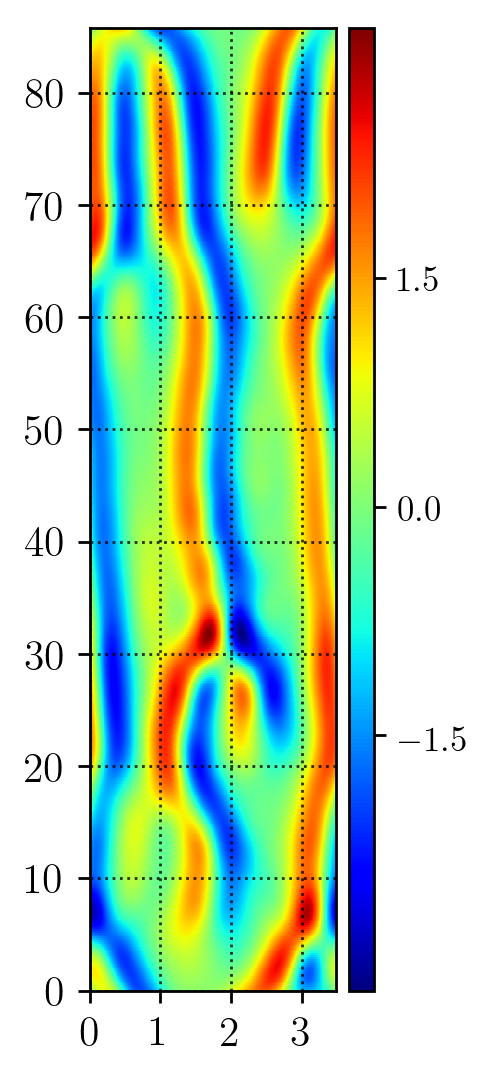
\includegraphics[width=.5\textwidth,height=.5\textheight]{MNG_halfdefect2_initial}
\end{minipage}
\begin{minipage}[height=.4\textheight]{.5\textwidth}
\centering
\small{\texttt{(b)}}\\
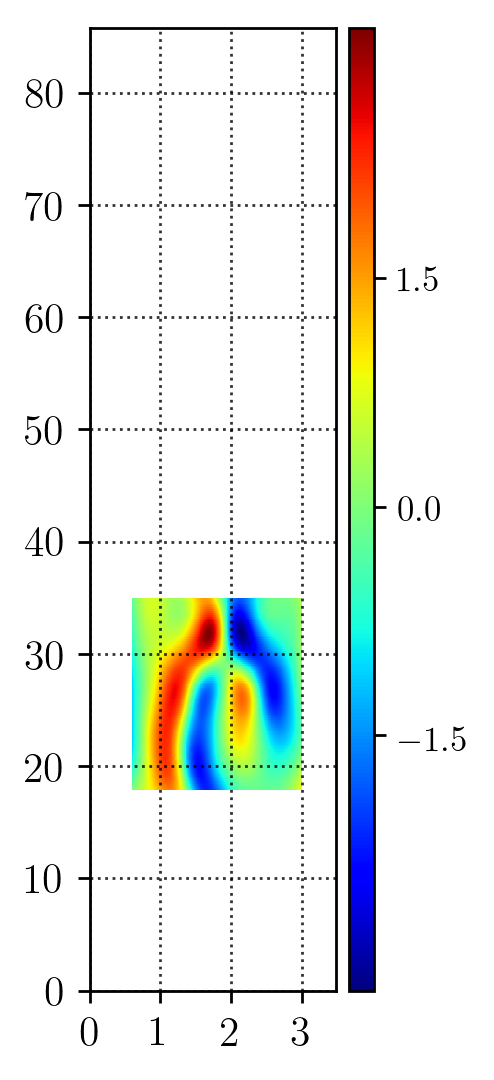
\includegraphics[width=.5\textwidth,height=.5\textheight]{MNG_halfdefect2_guess}
\end{minipage}
\begin{minipage}[height=.1\textheight]{\textwidth}
\centering
\small{\texttt{(c)}}\\
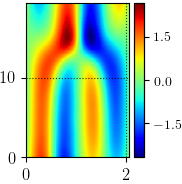
\includegraphics[width=.14\textwidth,height=.1\textheight]{MNG_halfdefect2}
\end{minipage}
\caption{ \label{fig:halfdefect2}
(a) \twoT\ with spatial translation symmetry defined on approximate domain $x \in [0,\approx 3.5(2\pi)]$, $t \in [0, \approx 85.735]$.  Truncation of significant digits is denoted by ``$\approx$'' .
(b) The extracted subdomain to serve as an
initial condition for tile searching. Defined on domain size $x \in [0,2.6(2\pi)]$, $t \in [0, 17]$.
}
\end{figure}

\begin{figure}
\begin{minipage}[height=.1\textheight]{.5\textwidth}
\centering
\small{\texttt{(a)}} \\
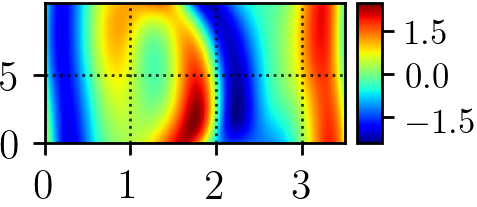
\includegraphics[width=.5\textwidth,height=.1\textheight]{MNG_hook_initial}
\end{minipage}
\begin{minipage}[height=.1\textheight]{.5\textwidth}
\centering
\small{\texttt{(b)}} \\
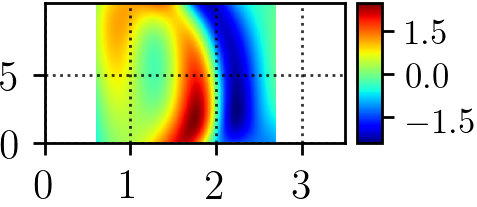
\includegraphics[width=.5\textwidth,height=.1\textheight]{MNG_hook_guess}
\end{minipage}
\begin{minipage}[height=.1\textheight]{\textwidth}
\centering
\small{\texttt{(c)}}\\
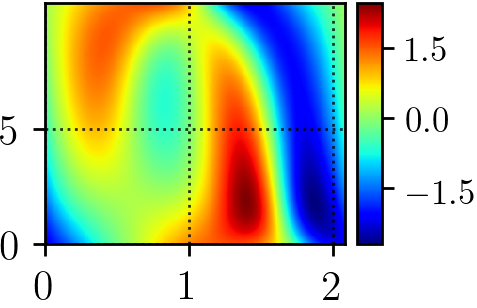
\includegraphics[width=.16\textwidth,height=.1\textheight]{MNG_hook}
\end{minipage}
\caption{ \label{fig:hook}
(a) Fundamental domain of \twoT\ with \spt\
shift-reflection symmetry defined on $x \in [0,\approx 3.5(2\pi)]$, $t \in [0, \approx 10.25]$.  Truncation of significant digits is denoted by ``$\approx$'' .
(b) The extracted subdomain to serve as an
initial condition for tile searching. Defined on domain size $x \in [0,2.1(2\pi)]$, $t \in [0, 10.5]$.
}
\end{figure}


\begin{figure}
\begin{minipage}[height=.3\textheight]{.5\textwidth}
\centering
\small{\texttt{(a)}} \\
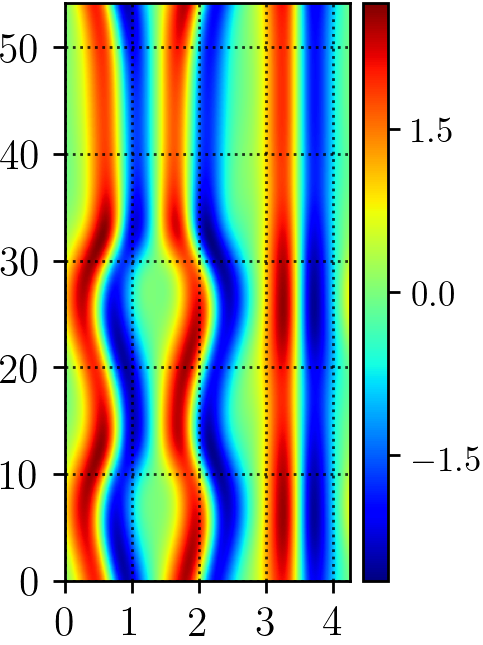
\includegraphics[width=.5\textwidth,height=.4\textheight]{MNG_gap_initial}
\end{minipage}
\begin{minipage}[height=.3\textheight]{.5\textwidth}
\centering
\small{\texttt{(b)}} \\
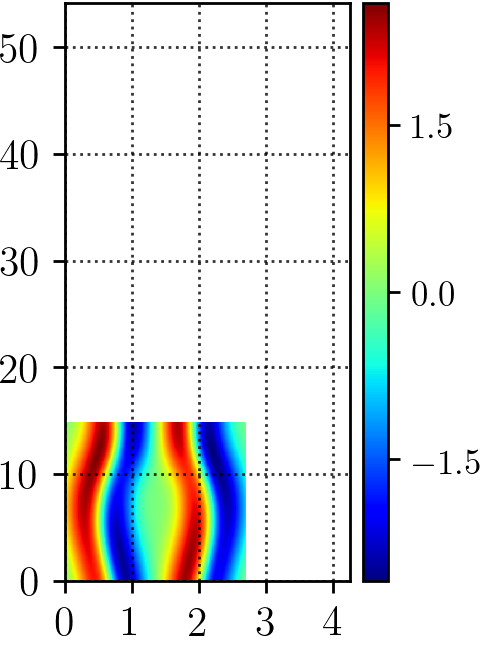
\includegraphics[width=.5\textwidth,height=.4\textheight]{MNG_gap_guess}
\end{minipage}
\begin{minipage}[height=.1\textheight]{\textwidth}
\centering
\small{\texttt{(c)}}\\
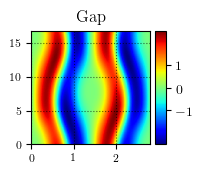
\includegraphics[width=.12\textwidth,height=.13\textheight]{MNG_gap}
\end{minipage}
\caption{ \label{fig:gap}
(a) \twoT\ defined on $x \in [0,\approx 4.25(2\pi)]$, $t \in [0, \approx 54.12]$.  Truncation of significant digits is denoted by ``$\approx$'' .
(b) The extracted subdomain to serve as an
initial condition for tile searching. Defined on domain size $x \in [0,2.7(2\pi)]$, $t \in [0, 15]$.
}
\end{figure}

\begin{figure}
\begin{minipage}[height=.4\textheight]{.5\textwidth}
\centering
\small{\texttt{(a)}} \\
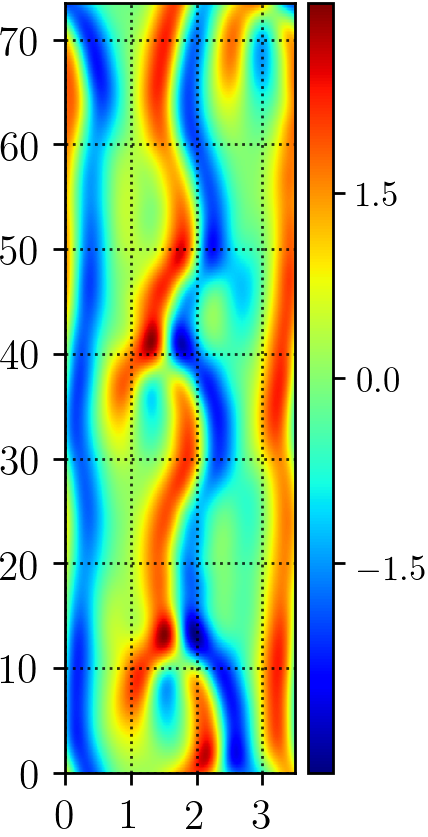
\includegraphics[width=.5\textwidth,height=.4\textheight]{MNG_hookondefect_initial}
\end{minipage}
\begin{minipage}[height=.4\textheight]{.5\textwidth}
\centering
\small{\texttt{(b)}} \\
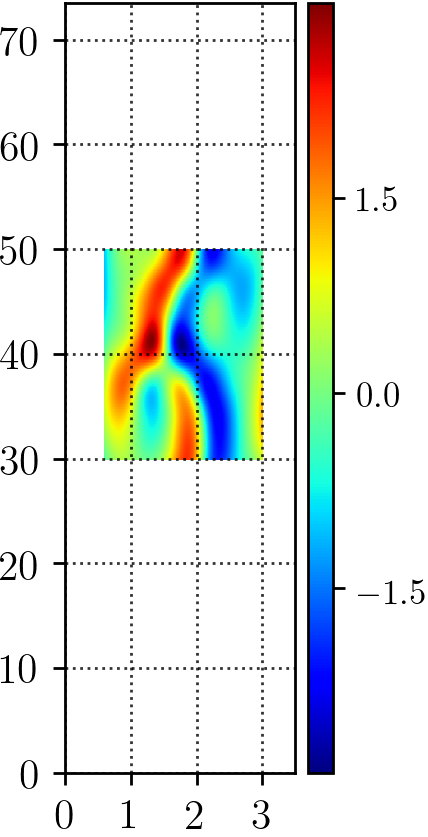
\includegraphics[width=.5\textwidth,height=.4\textheight]{MNG_hookondefect_guess}
\end{minipage}
\begin{minipage}[height=.4\textheight]{\textwidth}
\centering
\small{\texttt{(c)}} \\
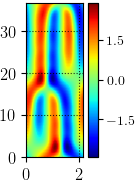
\includegraphics[width=.2\textwidth,height=.22\textheight]{MNG_hookondefect}
\end{minipage}
\caption{ \label{fig:hookondefect}
(a) Fundamental domain of \twot\ with \spt\
shift-reflection symmetry defined on $x \in [0,\approx 21.97]$, $t \in [0, \approx 73.52]$.  Truncation of significant digits is denoted by ``$\approx$'' .
(b) The extracted subdomain to serve as an
initial condition for tile searching. Defined on domain size $x \in [0,2.4(2\pi)]$, $t \in [0, 20]$. Both \reffig{fig:hookondefect2} (c) and \reffig{fig:hookondefect3}(c) demonstrate a similar pattern with similar \spt\ extent.
}
\end{figure}

\begin{figure}
\begin{minipage}[height=.4\textheight]{.5\textwidth}
\centering
\small{\texttt{(a)}} \\
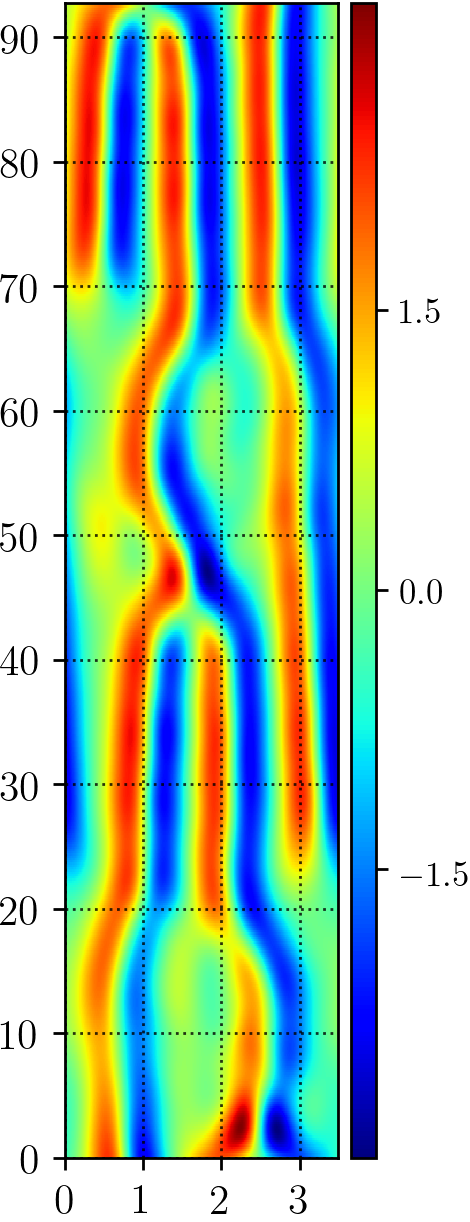
\includegraphics[width=.5\textwidth,height=.5\textheight]{MNG_hookondefect2_initial}
\end{minipage}
\begin{minipage}[height=.4\textheight]{.5\textwidth}
\centering
\small{\texttt{(b)}} \\
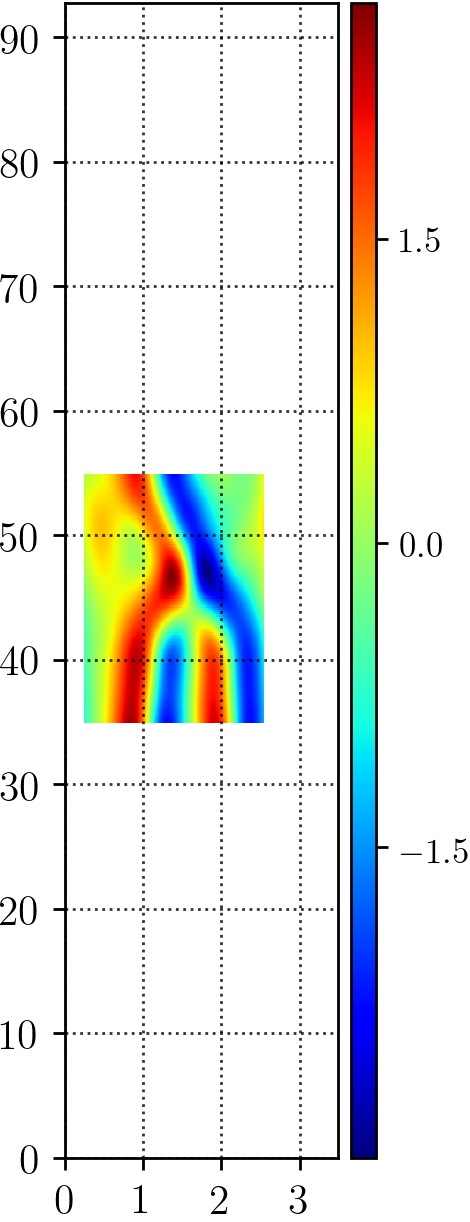
\includegraphics[width=.5\textwidth,height=.5\textheight]{MNG_hookondefect2_guess}
\end{minipage}
\begin{minipage}[height=.1\textheight]{\textwidth}
\centering
\small{\texttt{(c)}} \\
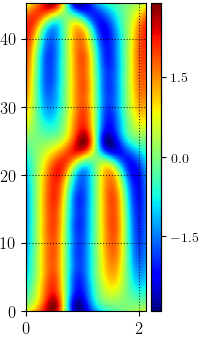
\includegraphics[width=.2\textwidth,height=.22\textheight]{MNG_hookondefect2}
\end{minipage}
\caption{ \label{fig:hookondefect2}
(a) Fundamental domain of \twoT\ with \spt\
shift-reflection symmetry defined on $x \in [0,\approx 21.93]$, $t \in [0, \approx 92.77]$.  Truncation of significant digits is denoted by ``$\approx$'' .
(b) The extracted subdomain to serve as an
initial condition for tile searching. Defined on domain size $x \in [0,2.3(2\pi)]$, $t \in [0, 20]$.
Both \reffig{fig:hookondefect}\,(c) and \reffig{fig:hookondefect3}\,(c) demonstrate a similar pattern with similar \spt\ extent.
}
\end{figure}

\begin{figure}
\begin{minipage}[height=.4\textheight]{.5\textwidth}
\centering
\small{\texttt{(a)}} \\
\includegraphics[width=.5\textwidth,height=.25\textheight]{MNG_hookondefect3_initial}
\end{minipage}
\begin{minipage}[height=.4\textheight]{.5\textwidth}
\centering
\small{\texttt{(b)}} \\
\includegraphics[width=.5\textwidth,height=.25\textheight]{MNG_hookondefect3_guess}
\end{minipage}
\begin{minipage}[height=.4\textheight]{\textwidth}
\centering
\small{\texttt{(c)}} \\
\includegraphics[width=.2\textwidth,height=.25\textheight]{MNG_hookondefect3}
\end{minipage}
\caption{ \label{fig:hookondefect3}
(a) Fundamental domain of \twoT\ with \spt\
shift-reflection symmetry defined on $x \in [0,\approx 21.99]$, $t \in [0, \approx 47.77]$.  Truncation of significant digits is denoted by ``$\approx$'' .
(b) The extracted subdomain to serve as an
initial condition for tile searching. Defined on domain size $x \in [0,2.5(2\pi)]$, $t \in [0, 25]$.
Both \reffig{fig:hookondefect}\,(c) and \reffig{fig:hookondefect2}\,(c) demonstrate a similar pattern with similar \spt\ extent.
}
\end{figure}

\begin{figure}
\begin{minipage}[height=.1\textheight]{.5\textwidth}
\centering
\small{\texttt{(a)}} \\
\includegraphics[width=.4\textwidth,height=.25\textheight]{MNG_321_initial}
\end{minipage}
\begin{minipage}[height=.1\textheight]{.5\textwidth}
\centering
\small{\texttt{(b)}} \\
\includegraphics[width=.4\textwidth,height=.2\textheight]{MNG_321}
\end{minipage}
\caption{ \label{fig:threeToone}
(a) Fundamental domain of \twoT\ with \spt\
shift-reflection symmetry defined on $x \in [0,\approx 3.5(2\pi)]$, $t \in [0, \approx 10.25]$.  Truncation of significant digits is denoted by ``$\approx$'' .
(b) The extracted subdomain to serve as an
initial condition for tile searching. Defined on domain size $x \in [0,2.1(2\pi)]$, $t \in [0, 10.5]$.
}
\end{figure}


\begin{figure}[t]
\begin{minipage}[height=.30\textheight]{.30\textwidth}
\centering
\includegraphics[width=1.0\textwidth]{MNG_01_initial}
\\ \small{\texttt{(a)}}
\end{minipage}
\begin{minipage}[height=.30\textheight]{.30\textwidth}
\centering \small{
\includegraphics[width=1.0\textwidth]{MNG_01_final}
\\ \small{\texttt{(c)}}}
\end{minipage}
\caption{\label{f:MNGtiling01none}
(a) Initial condition produced by taking defect and streak tiles,
padded them with zeros (spatiotemporally in a window-pane like
fashion), and then concatenating them. (b) The resulting
\spt\ field after being passed through adjoint descent. (c)
The fully converged solution, defined on $\conf \in [0,\approx 19.67
]$,$\zeit \in [0,\approx 20.84]$.
}
\end{figure}



\begin{figure}[t]
\begin{minipage}[height=.30\textheight]{.30\textwidth}
\centering
\includegraphics[width=1.0\textwidth]{MNG_001_initial}
\\ \small{\texttt{(a)}}
\end{minipage}
\begin{minipage}[height=.30\textheight]{.30\textwidth}
\centering \small{
\includegraphics[width=1.0\textwidth]{MNG_001_final}
\\ \small{\texttt{(b)}}}
\end{minipage}
\caption{\label{f:MNGtiling001none}
(a) Initial condition produced by taking one defect and two streak tiles,
padded them with zeros (spatiotemporally in a window-pane like
fashion), and then concatenating them spatially. (b) The resulting
\spt\ field after being passed through adjoint descent. (c)
The fully converged solution, defined on $\conf \in [0,\approx 25.90
]$,$\zeit \in [0,\approx 23.15]$.
}
\end{figure}

\begin{figure}[t]
\begin{minipage}[height=.30\textheight]{.30\textwidth}
\centering
\includegraphics[width=1.0\textwidth]{MNG_012_initial}
\\ \small{\texttt{(a)}}
\end{minipage}
\begin{minipage}[height=.30\textheight]{.30\textwidth}
\centering \small{
\includegraphics[width=1.0\textwidth]{MNG_012_final}
\\ \texttt{(b)}}
\end{minipage}
\caption{\label{f:MNGtiling012none}
(a) Initial condition produced by taking a single defect, gap, and streak tile,
padded them with zeros (spatiotemporally in a window-pane like
fashion), and then concatenating them spatially. (b) The resulting
\spt\ field after being passed through adjoint descent. (c)
The fully converged solution, defined on $\conf \in [0,\approx 39.98]$
,$\zeit \in [0,\approx 24.97]$.
}
\end{figure}


\MNGpost{2019-08-01}{:
As a preface to the following blog post:
for file names of tiling combinations,
zero refers to streak, one refers to defect
and two refers to gap. The format of
the filenames is as follows (examples that
have not been found yet)

The string \texttt{012 001} would represent
symbolic block, \ie the underscoring separates
the temporal portions of the blocks.

\beq
\Mm=\left[\begin{array}{c}
0 1 2 \\
0 0 1
\end{array}\right]
\eeq


All tilings (so far)
have assumed that the final solution has
no symmetries (its isotropy subgroup is
the trivial group).

Slightly worried
about tiling results. From the initial
conditions formed by simply zero-padding
and then concatenating tiles the solutions
(which have converged) look like they have
too much structure as compared to where
they initially begin. The result after
only the first numerical method,
adjoint descent, is more what I would think
the tiles should converge to. As can
be seen in \reffig{f:MNGtiling01none}.
Even though my expectations are being betrayed
it may just be a representation of the \spt\ grammar.

The streak defect spatial conjunction leads to
what I believe to be a representation of
a symbolic block of twice the temporal
extent as what I started with.
Specficically, I believe if I started
with

\beq
\Mm=\left[\begin{array}{c}
0 1
\end{array}\right]
\eeq

it ends up converging (after Gauss-Newton)
to the following

\beq
\Mm=\left[\begin{array}{c}
0 1^* \\
0 1
\end{array}\right]
\eeq

Now obviously this is undesirable
(if the targeted original symbolic block
is admissible). I don't mean to sound braggadocios
but perhaps this is due to the numerical methods
working \textit{too well}. Whether or not
the defect tile is in its comoving frame (because
its technically an \rpo\ with nearly a half-cell shift)
does not seem to affect what solution the initial conditions
converge to, up to spatial and temporal translations. I understand
that it makes no sense to join something which is in a co-moving
frame with something that is not, but this shows that
it doesn't seem to matter, numerically.

All of these facts seem to point to the fact that spatially
concatenating a defect to a streak is not admissible; only
the temporal concatenation (such that the result is a \ppo.)
seems to appear. The \ppo\ in question (or rather, representatives
of its continuous family) can be seen in part (c) of each
\reffig{fig:hookondefect},
\reffig{fig:hookondefect2}, and \reffig{fig:hookondefect3}.

This is also evidenced by \reffig{f:MNGtiling012none}
and \reffig{f:MNGtiling001none}.
}

\MNGpost{2019-08-05}{
Added a number of tiling results which were
found after some more tuning of the tiling methods.
In order to not miss certain admissible \spt\ symbolic
blocks, each symbolic block combination is looked for using
an array of different discretizations, specifically,
until a convergent solution is found (or until the available
discretizations are depleted). The initial
``minimum'' discretization (fewest number of points)
is given by  $N_{\text{min}}=\max (32,2^{\log_2(T)+1})$,
$M_{\text{min}}=\max(32,2^{\log_2(T)+1})$.
The range of discretizations is $N = N_{\text{min}},...,2*N_{\text{min}}$,
$M = M_{\text{min}},...,2*M_{\text{min}}$. These values are cycled
through in a two loop recursion incrementally increasing by 4.
The incremental increase (as opposed to a factor of 2 each time) is to
ensure that the discretizations do not get too large; a situation
which would eat up a gratuitous amount of computational time.

The solutions are always kept in a high resolution form
and then the rediscretization (truncation, if you would like to
think about it in \spt\ Fourier space) is applied at the beginning of
each trial. This ensures that we are not truncating and then interpolating,
merely truncating.

This helps convergence, but increases the
computation time as the number of trials increases. This and
other tuning efforts is the reason why I'm still working on
the $1 \times M$ sized tilings. The number of runs increasing
is taking a bit of time.

So far, after tuning, (a fancy way of saying trial \&
error) all tile combinations have been found when assuming
no symmetries; again, the issue lies in whether the final,
converged solutions actually pertain to the symbolic blocks in question.

Other than these tunings I've been getting back into improving
the numerical side of the code; just can't seem to get enough of it.

The future work other than
future tuning of the tiling; redoing the gluing method (similar
but not the same to tiling), more numerical methods, working
on the ``average spectrum'' initial conditions and
``seeding'' initial conditions, the latter is a process
of embedding tiles (or blocks) in a large \spt\ domain.

I'm hoping to get to either Kolmogorov flow or Navier-Stokes
doubly (triply) periodic flows before I leave; I could probably
start one of these when tiling code is finished.

Instead of dwelling on continuous improvement/optimization of \KS\ code
I'm going to try to move onto a harder problem once the tiling code is
exhausted.

I figure that my \KS\ code can be used as a testing ground for things that
I need to implement for Kolmogorov/Navier-Stokes doubly/triply periodic
flows. I have most of the machinery as I've tried to make the numerical
methods as modular as possible. (Literally just need to code Kolmogorov
functions for the spatiotemporal function, matrix vector product,
transpose matrix-vector product, FFTs).

This is, of course, as long as Predrag deems this appropriate; it seems
premature because the paper isn't done yet but I want to try my
hand at something new.
}

\PCpost{2019-08-06}{
What Predrag deems appropriate sounds like a broken record:
``The paper / thesis does not write itself''
``The paper / thesis does not write itself''
``The paper / thesis does not write itself''
``The paper / thesis does not write itself''
$\cdots$
``The paper / thesis does not write itself''

If you follow what is going on with \emph{kittens}, the other finished
project, REALLY writing a readable, publishable paper, with publishable
figures, correctly referenced and proofread always takes at least 3 times
longer than one had planned, and in the process one discovers that there
are many things one believed one understood, but did not, really.

At this point I would ration my time to 2/3rds paper / thesis writing,
1/3rd new research.
}

\MNGpost{2019-08-14}{
Added tiling figures and description to \texttt{tiles.tex}
demonstrating how one can tile the \spt\ state space
in a relatively straightforward manner, how it
links with symbolic dynamics. Need to
figure out how to describe the false positives
(\ie finding solutions not corresponding to original
tilings).

Splitting numerical methods descriptions to motivate
a much mroe in depth discussion regarding global
convergence properties, rates of convergence, etc.

}

\MNGpost{2019-08-15}{
Trying to expand the numerical methods section
to look more professional by looking at global
convergence and rates of convergence proofs
for Gauss-Newton methods such as in \rf{Schaback85}
but haven't found anything for adjoint descent.
Other, more commonly implemented
iterative methods like GMRES \rf{Saad1986}
have papers on the convergence properties such as
\rf{LieTic04} but they vary in how intelligible they
are, at least to me. I feel like
perhaps the ``adjoint descent method'' from \rf{Faraz15}
is perhaps a previously derived method under a different
name. Personally it seems too effective and
straightforward of a derivation (in the discretized case
it's just a fictitious time derivative of the cost
functional construction comprised of the $L_2$ norm
of the \spt\ ``Feynmann equation'' form of the \KSe.
It seems too straightforward to have not been done before.

Starting a subsection of variational that discusses
both the adjoint sensitivity analysis of \rf{Wang13} and \rf{Blonigan17}
and Hill's formula from \rf{BolTre10}.
}

\MNGpost{2019-08-19}{
Hessian of the \KSe\ Lagrangian take two.
in \texttt{variational.tex}
}

\MNGpost{2019-08-20}{
Expand \texttt{variational.tex}
via discussions regarding Hill's formula
\rf{BolTre10}, formal
Lagrangians \rf{Ibragimov10,IbragiKols04},
adjoint equations, adjoint sensitivity
formulas, least squares shadowing
\refrefs{Wang14,LaShMe18,Blonigan17,YSPS03,Gunzburger02},
calculus of variations and variational integrators
\refrefs{MPSW01,KraMaj15}.
}

\MNGpost{2019-08-21}{
\texttt{Variational.tex} started to
get too convoluted. Outline stated here for
writers benefit.

\begin{enumerate}
\item The point of transforming an IVP to a variational BVP
\item Introduction to variational notation
and variational calculus?
\item cost functional and action functional
\item alternative to stability, sensitivity
\item adjoint sensitivity
\item least-squares shadowing
\item hill's formula
\end{enumerate}
Read \rf{BoyVan04} to add details regarding
``least-norm optimization'' problems
}

\MNGpost{2019-08-22}{
Still fixing variational.tex

I want to be able to apply \rf{Ibragimov07a}
to the paper but I haven't figured it out yet;
I think perhaps if I use \rf{WeiWan19} as a guide
I can do it but will focus on writing for now.


}

\MNGpost{2019-08-24}{
Found \rf{liede} through references of
\rf{AncBlu97} which really inspired me to give
Lie Group analysis of \KSe\ and its (formal)
Lagrangian another go. Wrote a Mathematica script
to help in this regard; Everything is matching up this
time I just need a little more time to finish it up.

This and a few other resources which I will add soon
gave me some clarity into the steps I was missing
from papers such as \rf{IbragiKols04}. There was just
a few details I needed help on and \rf{liede} did the
trick I think.

In other news; I found a paper regarding a certain
explicit transformation that also applies to
the \KSe\ I believe which is possibly a different
way to handle Galilean velocity in the spirit of
Predrag's idea of matching tiles with said quantity
varying. Details in \rf{Miura68}, the concept is that
a generalized \KSe, with addition of a forcing term,
can be transformed back into the original \KSe (by the
same transformation they list for KdV). The specific
form of everything leads to the interpretation that
the forcing is due to the acceleration of the $\conf$ axis.
Which gives a transformation to an accelerating coordinate
frame as implied by the section title of the paper.
}


\MNGpost{2019-08-26}{
\begin{description}
\item[nonlinear transformation].
From \rf{Miura68}
The generalized \KSe\

\beq
u_t + u_{xx} + u_{xxxx} + u u_x = y_{tt}
\eeq

with notable time-dependent ``forcing term''
can be transformed back to the original \KSe\
via the set of transformations

\bea
t^{'} &=& t \continue
x^{'} &=& x - y(t) \continue
u(x,t) &=& u^{'}(x^{'},t^{'}) + y_{t^{'}}(t^{'})
\eea

back to the original \KSe\ in primed
variables.

Galilean transformations are a specific
example of this transformation as can
be readily seen by the substitution
$y(t) = v t$, $v$ being the Galilean
velocity.

\item[nonlinearly self-adjointness]
Following Ibragimov's idea of nonlinear
self adjointness, \ie\ set adjoint variable
equal to some arbitrary function of $u$ and
its derivatives and find solutions to the adjoint
equation.

Unfortunately the only solution is the constant
solution meaning that both the ``conservation law''
from \texttt{variational.tex} is trivial and always
satisfied so that the entire process is ostensibly worthless.
The only saving grace would be to look for variational
symmetries (symmetries of the Lagrangian itself as
opposed to equations), but \rf{liede} says that variational
symmetries (of a Lagrangian) are always symmetries of
the corresponding Euler-Lagrange equations, but not vice-versa.
Meaning, that we already have all symmetries of the governing
equations such that there are no alternative options.

It seems that the \KSe\ is just too simple (in terms of symmetries)
to benefit from this type of analysis. Note that we did not
investigate the role of parameters such as $T$ and $L$ as
thats not really the purview of this investigation.

In other words, this investigation that took quite a bit
of time for me to not only understand but implement in Mathematica
bore no fruit. In fact, there isn't even a tree for said fruit.
\end{description}
}

\MNGpost{2019-08-27}{
Variational stuff copied from \texttt{variational.tex}

\beq
\mathbf{\text{pr}} v^{(4)} = \epsilon(x,t,u)\frac{\partial}{\partial x}
+\tau(x,t,u)\frac{\partial}{\partial t}
+\phi(x,t,u)\frac{\partial}{\partial u}
+\phi^t(x,t,u^{(1)})\frac{\partial}{\partial u_t}
+\phi^x(x,t,u^{(1)})\frac{\partial}{\partial u_x}
+\phi^{xx}(x,t,u^{(2)})\frac{\partial}{\partial u_{xx}}
+\phi^{xxxx}(x,t,u^{(4)})\frac{\partial}{\partial u_{xxxx}}\,,
\eeq

because all other terms will annihilate when
acting on the \KSe. Note that the higher the order of the
coefficient the more terms it depends on due to the
differentiation that takes place in \refeq{e-vectorcoeff}

Now that we have the general
form of the vector field we can begin to derive
the \textit{infinitesimal generators} which span
the Lie algebra. To accomplish this, we will derive
the \textit{determining equations} which are produced
by applying \refeq{e-vectorfield} to the system of differential
equations and equating to zero, that is

\beq
\mathbf{\text{pr}} v^{(4)}(G(u^(\alpha)(\conf,\zeit),u_{(1)}^(\alpha)(\conf,\zeit),\dots,u_{(n)}^(\alpha)(\conf,\zeit))) = 0
\eeq

performing this operation yields the following equation

\beq \label{e-KSEcoeff}
\phi^t + \phi^{xx} + \phi^{xxxx} + u \phi^x + \phi u_x = 0 \,.
\eeq

We finally are forced to derive the coefficients $\phi^J$
and to include as many details as possible
we will write the exact formulas needed to derive them
as well as the long form expressions that they are equal to.

\bea
\phi^t &=& D_t (\phi(x,t,u) -\epsilon(x,t,u) u_x -\tau(x,t,u) u_t) + \tau(x,t,u) u_tt + \epsilon(x,t,u) u_xt \continue
\phi^x &=& D_x (\phi(x,t,u) -\epsilon(x,t,u) u_x -\tau(x,t,u) u_t) + \tau(x,t,u) u_tx + \epsilon(x,t,u) u_xx  \continue
\phi^{xx} &=& D_{x}^2 (\phi(x,t,u) -\epsilon(x,t,u) u_x -\tau(x,t,u) u_t) + \tau(x,t,u) u_{txx} + \epsilon(x,t,u) u_{xxx} \continue
\phi^{xxxx} &=& D_{x}^4 (\phi(x,t,u) -\epsilon(x,t,u) u_x -\tau(x,t,u) u_t) + \tau(x,t,u) u_{txxx} + \epsilon(x,t,u) u_{xxxx}
\eea

where $D_t$ and $D_x$ represent \textit{total differentiation} operators,

\beq
D_i = \frac{\partial}{\partial x^i} + u_i \frac{\partial}{\partial u} + u_{ii} \frac{\partial}{\partial u_i} + \dots
\eeq

the long form expressions from each of these are
\beq
\phi ^t=u_t^2 \left(-\tau _u\right)-\tau _t u_t-u_t u_x \epsilon _u-\epsilon _t u_x+u_t \phi _u+\phi _t
\eeq

\beq
\phi ^x=-u_t \tau _u u_x-u_t \tau _x+u_x^2 \left(-\epsilon _u\right)-u_x \epsilon _x+u_x \phi _u+\phi _x
\eeq

\bea
\phi ^{\text{xx}}&=&-u_t u_x^2 \tau _{\text{uu}}-2 u_t u_x \tau _{\text{xu}}-u_t \tau _u u_{\text{xx}}\continue
&-&u_t \tau _{\text{xx}}+u_x^3 \left(-\epsilon _{\text{uu}}\right)+u_x^2 \phi _{\text{uu}}\continue
&-&2 \tau _u u_x u_{\text{xt}}-2 u_{\text{xt}} \tau _x-2 u_x^2 \epsilon _{\text{xu}}\continue
&+&2 u_x \phi _{\text{xu}}-3 u_x u_{\text{xx}} \epsilon _u-u_x \epsilon _{\text{xx}}\continue
&-&2 u_{\text{xx}} \epsilon _x+u_{\text{xx}} \phi _u+\phi _{\text{xx}}
\eea

\bea
\phi ^{\text{xxxx}}&=&-4 u_t u_x u_{\text{xxx}} \tau _{\text{uu}}-3 u_t u_{\text{xx}}^2 \tau _{\text{uu}}-6 u_t u_x^2 u_{\text{xx}} \tau _{\text{uuu}}-u_t u_x^4 \tau _{\text{uuuu}} \continue
&-&12 u_t u_x u_{\text{xx}} \tau _{\text{xuu}}-4 u_t u_x^3 \tau _{\text{xuuu}}-6 u_t u_x^2 \tau _{\text{xxuu}}-4 u_t u_x \tau _{\text{xxxu}}-4 u_t u_{\text{xxx}} \tau _{\text{xu}}\continue
&-&6 u_t u_{\text{xx}} \tau _{\text{xxu}}-u_t \tau _u u_{\text{xxxx}}-u_t \tau _{\text{xxxx}}-12 u_x u_{\text{xt}} u_{\text{xx}} \tau _{\text{uu}} \continue
&-&15 u_x u_{\text{xx}}^2 \epsilon _{\text{uu}}-6 u_x^2 u_{\text{xxt}} \tau _{\text{uu}}-10 u_x^2 u_{\text{xxx}} \epsilon _{\text{uu}}+4 u_x u_{\text{xxx}} \phi _{\text{uu}} \continue
&+&3 u_{\text{xx}}^2 \phi _{\text{uu}}-4 u_x^3 u_{\text{xt}} \tau _{\text{uuu}}-10 u_x^3 u_{\text{xx}} \epsilon _{\text{uuu}}+6 u_x^2 u_{\text{xx}} \phi _{\text{uuu}}\continue
&+&u_x^5 \left(-\epsilon _{\text{uuuu}}\right)+u_x^4 \phi _{\text{uuuu}}-12 u_x^2 u_{\text{xt}} \tau _{\text{xuu}}-12 u_x u_{\text{xt}} \tau _{\text{xxu}}\continue
&-&12 u_x u_{\text{xxt}} \tau _{\text{xu}}-16 u_x u_{\text{xxx}} \epsilon _{\text{xu}}-24 u_x^2 u_{\text{xx}} \epsilon _{\text{xuu}}+12 u_x u_{\text{xx}} \phi _{\text{xuu}}\continue
&-&4 u_x^4 \epsilon _{\text{xuuu}}+4 u_x^3 \phi _{\text{xuuu}}-18 u_x u_{\text{xx}} \epsilon _{\text{xxu}}-6 u_x^3 \epsilon _{\text{xxuu}}+6 u_x^2 \phi _{\text{xxuu}}\continue
&-&4 \tau _u u_x u_{\text{xxxt}}-4 u_{\text{xxxt}} \tau _x-4 u_x^2 \epsilon _{\text{xxxu}}+4 u_x \phi _{\text{xxxu}}-5 u_x u_{\text{xxxx}} \epsilon _u-u_x \epsilon _{\text{xxxx}}\continue
&-&4 u_{\text{xxxx}} \epsilon _x-12 u_{\text{xt}} u_{\text{xx}} \tau _{\text{xu}}-4 \tau _u u_{\text{xt}} u_{\text{xxx}}-4 u_{\text{xt}} \tau _{\text{xxx}}\continue
&-&12 u_{\text{xx}}^2 \epsilon _{\text{xu}}+4 u_{\text{xxx}} \phi _{\text{xu}}-6 \tau _u u_{\text{xx}} u_{\text{xxt}}-6 u_{\text{xxt}} \tau _{\text{xx}}\continue
&+&6 u_{\text{xx}} \phi _{\text{xxu}}-10 u_{\text{xx}} u_{\text{xxx}} \epsilon _u-6 u_{\text{xxx}} \epsilon _{\text{xx}}-4 u_{\text{xx}} \epsilon _{\text{xxx}}\continue
&+&u_{\text{xxxx}} \phi _u+\phi _{\text{xxxx}}
\eea

upon substitution into \refeq{e-KSEcoeff} we can separate the terms by coefficients
of monomials which gives us the determining equations as previously mentioned
\beq
\begin{array}{c}
 \phi _t+\phi _{\text{xx}}+\phi _{\text{xxxx}}=0 \\
 -4 \tau _x=0 \\
 -6 \tau _{\text{xx}}=0 \\
 -2 \tau _x-4 \tau _{\text{xxx}}=0 \\
 -4 \epsilon _x+\tau _t+\tau _{\text{xx}}+\tau _{\text{xxxx}}=0 \\
 4 \phi _{\text{xu}}-6 \epsilon _{\text{xx}}=0 \\
 -4 \tau _u=0 \\
 4 \tau _{\text{xu}}=0 \\
 -2 \epsilon _x-4 \epsilon _{\text{xxx}}+\tau _t+\tau _{\text{xx}}+\tau _{\text{xxxx}}+6 \phi _{\text{xxu}}=0 \\
 -6 \tau _u=0 \\
 -12 \tau _{\text{xu}}=0 \\
 6 \tau _{\text{xxu}}=0 \\
 4 \tau _{\text{xu}}-10 \epsilon _u=0 \\
 -12 \epsilon _{\text{xu}}+6 \tau _{\text{xxu}}+3 \phi _{\text{uu}}=0 \\
 3 \tau _{\text{uu}}=0 \\
 3 \tau _{\text{uu}}=0 \\
 \phi -\epsilon _t-\epsilon _{\text{xx}}-\epsilon _{\text{xxxx}}+2 \phi _{\text{xu}}+4 \phi _{\text{xxxu}}=0 \\
 -4 \tau _u=0 \\
 -12 \tau _{\text{xu}}=0 \\
 -2 \tau _u-12 \tau _{\text{xxu}}=0 \\
 -4 \epsilon _u+2 \tau _{\text{xu}}+4 \tau _{\text{xxxu}}=0 \\
 4 \phi _{\text{uu}}-16 \epsilon _{\text{xu}}=0 \\
 4 \tau _{\text{uu}}=0 \\
 -2 \epsilon _u-18 \epsilon _{\text{xxu}}+2 \tau _{\text{xu}}+4 \tau _{\text{xxxu}}+12 \phi _{\text{xuu}}=0 \\
 -12 \tau _{\text{uu}}=0 \\
 12 \tau _{\text{xuu}}=0 \\
 4 \tau _{\text{uu}}=0 \\
 12 \tau _{\text{xuu}}-15 \epsilon _{\text{uu}}=0 \\
 -2 \epsilon _{\text{xu}}-4 \epsilon _{\text{xxxu}}+\phi _{\text{uu}}+6 \phi _{\text{xxuu}}=0 \\
 -6 \tau _{\text{uu}}=0 \\
 -12 \tau _{\text{xuu}}=0 \\
\end{array}
\eeq

\beq \nonumber
\begin{array}{c}
 \tau _{\text{uu}}+6 \tau _{\text{xxuu}}=0 \\
 -10 \epsilon _{\text{uu}}=0 \\
 -24 \epsilon _{\text{xuu}}+\tau _{\text{uu}}+6 \tau _{\text{xxuu}}+6 \phi _{\text{uuu}}=0 \\
 6 \tau _{\text{uuu}}=0 \\
 6 \tau _{\text{uuu}}=0 \\
 -\epsilon _{\text{uu}}-6 \epsilon _{\text{xxuu}}+4 \phi _{\text{xuuu}}=0 \\
 -4 \tau _{\text{uuu}}=0 \\
 4 \tau _{\text{xuuu}}=0 \\
 4 \tau _{\text{xuuu}}-10 \epsilon _{\text{uuu}}=0 \\
 \phi _{\text{uuuu}}-4 \epsilon _{\text{xuuu}}=0 \\
 \tau _{\text{uuuu}}=0 \\
 \tau _{\text{uuuu}}=0 \\
 -\epsilon _{\text{uuuu}}=0 \\
 \phi _x=0 \\
 \tau _x=0 \\
 \tau _x=0 \\
 -\epsilon _x+\tau _t+\tau _{\text{xx}}+\tau _{\text{xxxx}}=0 \\
 4 \tau _{\text{xu}}=0 \\
 6 \tau _{\text{xxu}}=0 \\
 3 \tau _{\text{uu}}=0 \\
 2 \tau _{\text{xu}}+4 \tau _{\text{xxxu}}=0 \\
 4 \tau _{\text{uu}}=0 \\
 12 \tau _{\text{xuu}}=0 \\
 \tau _{\text{uu}}+6 \tau _{\text{xxuu}}=0 \\
 6 \tau _{\text{uuu}}=0 \\
 4 \tau _{\text{xuuu}}=0 \\
 \tau _{\text{uuuu}}=0 \\
 \tau _x=0 \\
\end{array}
\eeq

While initially intimidating, these equations can be solved by noticing
the lower order equations such as $\tau_x = \tau_u = 0$ which means
that $\tau$ can only be a function of $t$. Following this reasoning
we find that in fact

\bea
\tau(x,t,u) &=& \tau = c_1 \continue
\epsilon(x,t,u)&=&\epsilon(t)= c_3 t + c_1 \continue
\phi(x,t,u)&=& \phi = c_3
\eea

such that the Lie algebra of infinitesimal symmetries
is spanned by
\bea \label{e-ksegenerators}
v_1 &=& \partial_x \continue
v_2 &=& \partial_t \continue
v_3 &=& t \partial_x + \partial_u
\eea

which are the generators of space and time translations as well as Galilean
transformations. This is not surprising as these symmetries are well
known \rf{BudCvi14} but we need to know the prolongations of \refeq{e-ksegenerators}
and their extensions to the adjoint variables present in \refeq{e-implicitadjoint}.

The prolongations of \refeq{e-ksegenerators} results in
\bea \label{e-ksegeneratorsprolong}
\mathbf{\text{pr}} v_1 &=& y_1 = \partial_x \continue
\mathbf{\text{pr}} v_2 &=& y_2 = \partial_t \continue
\mathbf{\text{pr}} v_3 &=& y_3 = \partial_x + \partial_u - u_x \partial_{u_t}\,.
\eea

We can now derive the extended versions of \refeq{e-ksegeneraorsprolong}
such that we can apply them to the formal Lagrangian \refeq{e-formallagrangian}
Once again we follow the machinery of Ibragimov to extend \refeq{e-ksegeneratorsprolong}
to the adjoint variables. Unfortunately it seems that the symmetries were too simple
to actually have extensions to the adjoint variables, but we can still go forward with
the conservation law calculations regardless. Both \rf{Ibragimov07a} and \rf{liede}
both work through the proof that there is a conserved vector (as Ibragimov calls it)
such that its divergence provides a conservation law (technically infinite number
of conservation laws because they are equations involving PDE solutions). The components
of the conserved vector (one for each independent variable) are given by

\beq
C^i = \xi^i \mathcal{L} + W^{\alpha}[\frac{\partial \mathcal{L}}{\partial u^{\alpha}_i}-D_j \frac{\partial \mathcal{L}}{\partial u^{\alpha}_{ij}}
+D_j D_k \frac{\partial \mathcal{L}}{\partial u^{\alpha}_{ijk}} - +D_j D_k D_l \frac{\partial \mathcal{L}}{\partial u^{\alpha}_{ijkl}}]
+ D_j(W^{\alpha})[\frac{\partial \mathcal{L}}{\partial u^{\alpha}_{ij}}-D_k \frac{\partial \mathcal{L}}{\partial u^{\alpha}_{ijk}}
+D_k D_l \frac{\partial \mathcal{L}}{\partial u^{\alpha}_{ijkl}}]
+ D_j D_k (W^{\alpha})[\frac{\partial \mathcal{L}}{\partial u^{\alpha}_{ijk}}-D_l \frac{\partial \mathcal{L}}{\partial u^{\alpha}_{ijkl}}
+D_k D_j \frac{\partial \mathcal{L}}{\partial u^{\alpha}_{ikj}} - +D_k D_j D_l \frac{\partial \mathcal{L}}{\partial u^{\alpha}_{ikjl}}]
+ D_j D_k D_l (W^{\alpha})[\frac{\partial \mathcal{L}}{\partial u^{\alpha}_{ijkl}}]\,,
\eeq

where the equation has been extended to include all possible non-zero terms in the context of the \KSe, $W^{\alpha}$ is shorthand
for $\phi^{\alpha} + \xi^i u_i^{\alpha}$. Applying this to our generators
yields one unique conservation law which we shall now detail.

For the Galilean transformation generator $\mathbf{\text{pr}} v_3 = t \partial_x + \partial_u -u_x \partial_{u_t}$
the components equal
\bea
C^x &=& t*\mathcal{L} + W[\frac{\partial \mathcal{L}}{\partial u_x}-D_x\frac{\partial \mathcal{L}}{\partial u_{xx}}-D_x^3\frac{\partial \mathcal{L}}{\partial u_{xxxx}}] \continue
    &+& D_x(W)[\frac{\partial \mathcal{L}}{\partial u_{xx}}+D_x^2\frac{\partial \mathcal{L}}{\partial u_{xxxx}}]\continue
    &+& D_x^2(W)[-D_x\frac{\partial \mathcal{L}}{\partial u_{xxxx}}]\continue
    &+& D_x^3(W)[\frac{\partial \mathcal{L}}{\partial u_{xxxx}}]\continue
C^t &=& 0*\mathcal{L} + (1-tu_x)[\frac{\partial \mathcal{L}}{\partial u_t}]
\eea

which both simplify to

\bea
C^x &=& t(u_tv+u_xv_x+u_xv_{xxx}+u_{xxx}v_x+u_{xx}v_{xx})+uv-v_x-v_{xxx} \continue
C^t &=& v_t - v u_x - u_x v_t t
\eea

such that the conservation law is given by the divergence
\bea
D_x (C^x) + D_t (C^t) &=& 0 \continue
                      &=& v_t - v u_x - u_x v_t t + uv_x +vu_x - v_{xx} - v_{xxxx}\continue
                      &+& t(v_x(u_t+u_{xx}+u_{xxxx})+u_x(v_xx+v_xxxx)+2D_x(u_{xx}v_{xx}))\continue
                      &=&t(v_x(u_t+u_{xx}+u_{xxxx})+u_x(-v_t+v_{xx}+v_{xxxx})++2D_x(u_{xx}v_{xx}))\continue
                      &=&2D_x(u_{xx}v_{xx})\,.
\eea

where multiple times we have substituted one of the equations from \refeq{e-optimalitysystem}.

The conserved quantity
\beq
D_x(u_{xx}v_{xx}) = 0
\eeq

Or upon integration (note: there is implicit time dependence)
\beq
u_{xx}v{xx} = y(t)
\eeq


Following the analysis of Burgers' equation and
the prescription of \rf{IbragiKols04}
we find an alternative form of the Lagrangian for the \KSe\ to be


There are various choices for
For instance, if upon substitution $v=u$ into the adjoint equation
reproduces the original equation, the equation is said to be
\textit{self-adjoint}.
Introduced in \rf{Ibragimov10} there are the notions of self-adjoint, quasi-self-adjoint
and nonlinearly-adjoint equations.

}

\MNGpost{2019-08-27}{
I was being stubborn and had an idea regarding the variational stuff.
I thought the adjoint variable
$v(x,t) = u(-x,-t) = R_x R_t u(x,t)$ given by space and time reflections
would solve the adjoint equation as it would flip the sign on the single
derivative times but after wasting some time I realized
this type of answer could never work due to the presence of $u(x,t)$ in
the adjoint equations. In other words, I would retrieve
something very close to the \KSe\ but not exactly it; therefore not being an answer.

}

\MNGpost{2019-08-29}{
Investigations into the rate of convergence
of the adjoint descent method and just adjoint
methods in optimization in general have lead to
the revelation that the adjoint descent method, when
applied to my \spt\ problem at least, is merely
the steepest descent algorithm applied to the
cost functional $\mathcal{L} = 1/2 ||F||^2$.

The derivation was written in \texttt{adjointdescent.tex}.
This means that there should be
room for numerical improvements.
}

\MNGpost{2019-09-09}{
Crunch time as the September 30th deadline is fast approaching

Focusing on expanding the writing in \texttt{trawl.tex},
\texttt{tiles.tex},\texttt{glue.tex} (the results basically).

I wish I had more time because my codes need to be refactored
yet again because they are simply getting too large and convoluted;
I began the process but the shift is so large I am keeping
all records of my work on github and trying to keep this
as a tertiary, weekend job.

The goal is to completely revamp the project (and as a symbolic
action I am going to rename the project to ``torihunter''.)
to be much more object oriented. Currently it takes a rather intimate
knowledge of the package to be able to write scripts, and it is
also specific to the \KSe. By switching to object oriented
programming, a general ``Torus'' class can be instantiated
such that instead of using specific functions, general class
methods can be used (basically the way to go about it is
to pass functions as a class method. The general idea is that
we should be able to pass \textit{any} Jacobian and spatiotemporal
function and have the numerical methods work, not just ones specific to
the \KSe). The manner by which to pass \spt\ symmetry constraints (on the Fourier modes,
I mean) is to have this built into the functions themselves.
}

\MNGpost{2019-09-11}{
Writing and running scripts which quantify the
dependence on the size of the \spt\ discretization.
Specifically I'm going to do two things. Produce
plots that demonstrate the rate of convergence
depending on $N,M$ for various $L,T$. Also,
for some given initial conditions known to converge at $\tilde{N},\tilde{M}$,
investigate the rate of convergence for $N_i,M_i < \tilde{N},\tilde{M}$,
to see if this informs us on how to minimize $N,M$.
This information will go into \texttt{trawl.tex} as it is regarding the finding
of solutions.
}

\MNGpost{2019-09-12}{
Migrated \texttt{variational.tex} Ibragimov stuff to\\ \texttt{LieGroupAnalysis.tex}
More \texttt{trawl.tex} edits, more work on\\ \texttt{convergence\_rate.py} to
produce analyses on discretization sizes.
}

\MNGpost{2019-09-23}{
Got lost in the weeds trying to see if I could apply machine learning
to find the ``faces'' of the \KSe. Specifically, ``Gabor wavelets''  (just a modulated Gaussian in
two dimensions) \rf{Lee96} can be used as image processing filter and pick out
``features'' which can be applied to facial recognition \rf{LBPA01}.

Started to write ideas relating the \spt\ continuation methods to demonstrate
how useful they are in the plumber's world. The basic benefits are
\begin{enumerate}
\item Reynolds number continuation to compare and reproduce data
\item Domain size continuation to compare and reproduce data
\item Geometry continuation? (maybe? likely very very ill conditioned)
\item Able to transform data to match experiments. Idea is that one of
the most common things to change in experimental setup is the size
of spatial domains.
\item Being able to analyze the full \spt\ state space of all parameter
values (as dictated by equations) instead of mistaking a tree for the forest.
\end{enumerate}
}

\begin{figure}[t]
\begin{minipage}[height=.30\textheight]{.30\textwidth}
\centering
\includegraphics[width=1.0\textwidth]{MNG_block}
\\ \small{\texttt{(a)}}
\end{minipage}
\begin{minipage}[height=.30\textheight]{.30\textwidth}
\centering \small{
\includegraphics[width=1.0\textwidth]{MNG_peakmax}
\\ \texttt{(b)}}
\end{minipage}
\caption{\label{f:MNGpeakmax}
(a) \twoT\ converged in full state space purported to be
symbolic block $1012$ (spatial sequence)
%$[\speriod{a},\period{a}]=[8.19\cdots, 37.45\cdots]$.
(b)Local maxima peak detection of (a) using skimage package.
}
\end{figure}

\begin{figure}[t]
\begin{minipage}[height=.80\textheight]{.80\textwidth}
\centering
\includegraphics[width=1.0\textwidth]{MNG_peakmax_orb}
\end{minipage}
\caption{\label{f:featuredetectpeakmax}
(a) Feature detection ``ORB'' routine applied to
\reffig{f:MNGpeakmax}(b).}
\end{figure}

\begin{figure}[t]
\begin{minipage}[height=.50\textheight]{.80\textwidth}
\centering
\includegraphics[width=1.0\textwidth]{MNG_peakmax_dots}
\\ \small{\texttt{(a)}}
\end{minipage}
\caption{\label{f:MNGpeakmaxdots}
 The ``detected'' points indicating features in the
image data (without parameter tuning)s.
}
\end{figure}


%\begin{figure}[t]
%\begin{minipage}[height=.30\textheight]{.30\textwidth}
%\centering
%\includegraphics[width=1.0\textwidth]{MNG_largeux_orb}
%\\ \small{\texttt{(a)}}
%\end{minipage}
%\begin{minipage}[height=.30\textheight]{.30\textwidth}
%\centering \small{
%\includegraphics[width=1.0\textwidth]{MNG_largeux_dots}
%\\ \texttt{(b)}}
%\end{minipage}
%\caption{\label{f:featuredetectlargeST}
%(a) Feature detection algorithm applied to th
%}
%\end{figure}


\MNGpost{2019-09-23}{
Further investigation into image processing in the spirit of facial recognition
of the ``faces'' of the \KSe. There are of course many many things to take
into account but the main goal of this was to create a way to detect tiles
embedded in shadowing orbits. Partial success so far; although features can be detected
I haven't figured out a way to classify them numerically; I have a good idea for how
to do so manually however.

If one takes any solution to the \KSe, \twot\ or otherwise; and passes it through a image
processing routine which picks out the local maxima based on image data alone (easier
that making mistakes and trying to implement by hand, using skimage Python package).
This produces \reffig{f:MNGpeakmax} which demonstrates what picking out the local maxima
would look like. The results (with these parameters, to be specific) are quite striking.
Recall that we're using these methods to detect features which correspond to tiles.
It appears in \reffig{f:MNGpeakmax}(b) that streaks are represented by, well, streaks. \textit{New} streaks however
leave a signature of
an upwards facing pitchfork, while mergers are represented by downward facing pitchforks (in this case there
is an example of an ``imperfect pitchfork'' like from bifurcation theory). There is a thick wishbone type shape
which represents a gap and an annulus on the left side on the domain which appears to represent either a hook (member of the
merger tile family) or another gap; this is hard to distinguish because of boundary effects.

The reason why these features are useful is because we can categorize all members of the tile continuous
families with one distinct shape even more distinct than the color coded tiles.
Using these shapes as indicators, I believe we may confidently say that this tile is not a
representation of the spatial sequence $1012$ as previously believed. Venturing a guess; this is
a much more complicated such as
\beq
\Mm=\left[\begin{array}{c}
0\,0\,0\,0\,0\,0\,0 \\
2\,2\,2\,2\,0\,0\,0 \\
0\,1\,0\,1\,0\,0\,0
0\,0\,0\,0\,0\,0\,0
\end{array}\right]
\ee{e-new1012blockguess}
but this is a quick guess.s

Let us assume that these categorizations using new codes are valid; how do we use them?
Luckily for us there is already code which can be used for feature detection; that is,
it picks out features in images that are robust under affine transformations and scalings
(they can be detected before and after the transformation, that is).

A beginner's level application of the feature detecting routines provides at least some
``detections'' around the key features described previously (upward/downward pitchfork, streaks, etc.).
This can likely be tuned to reduce the number of detections of streaks; this is desireable
because if we find the number (and location) of gaps and mergers, we can fill out the rest
of the \twot\ with streaks.

The \texttt{.png} files used in \reffig{f:MNGpeakmax} are kept as large files for future use,
as these methods directly use image data.
}

\MNGpost{2019-10-11}{
I tried to derive a clean result for the \spt\ \KSe\ which follows
the course of action of Predrag's stability derivation but the results
are inconsistent with the stability properties of the tests performed with
$L=22$ orbits with well known stability properties.

I will walk through the derivation now and hopefully someone can tell me where I
have gone wrong. I work in \spt\ Fourier space because not only is it
most familiar but also I wanted to investigate spatial stability
as well.
We begin with the analog of the vector $\hat{p}$ which instead of a collection
of state-space points we have a finite dimensional representation of the infinite
dimensional scalar field $u(x,t)$ in \spt\ Fourier space. I will label the
\spt\ modes by $\tilde{u}_{kj}$, $k$ for space and $j$ for time. I'm using the convention
$u(x_m,t_n)\equiv u_n$ for time indices to simplify the
expressions. We can use an analog of the multishooting difference function
$F$ \refeq{errorVecs1D}.
\beq
 F(\hat{u})
=
\begin{array}{c}
\hat{u} - g \circ (\hat{u} + v(\hat{u})\delta t)
\end{array}
\eeq
Put very simply, this maps the field, reorders it, and then
subtracts it from the original. The indices for both terms are now the
same thanks to the rotation; there are implied indices which correspond to
 $\conf_m$ and $\zeit_n$
The reason that I pursued a form was because I thought that I could make a
block diagonal if not diagonal form. My original error was that I thought I
could make use of the
spectral differentiation operator
$\hat{u}_t = \sum_{k,j} i w_j \hat{\tilde{u}}_{k,j} e^{i (w_j t_n + q_k x_m)}$.
This is equivalent to multiplication by a diagonal matrix whose diagonal
is $k$ copies of $i w_j$. The problem with this is that yes; it produces the exact
same velocity field $u_t = -u_{xx} -u_{xxxx} - u u_x$ but the linearization is not
at all the same and as such gives us a nonsensical \jMps which doesn't even depend
on $\tilde{u}$. This was clearly wrong; substitution of
$u_t = -u_{xx} -u_{xxxx} - u u_x$ yields
%
\beq
 F(\hat{u})
=
\begin{array}{c}
\tilde{u}_{k,j} - \exp^{i w_j \delta t} (\tilde{u}_{k,j} + [(q_k^2 - q_k^4) \tilde{u}_{k,j}
+ \frac{iq_k}{2} \mathcal{F}(\mathcal{F}^{-1}\tilde{u}_{k,j})^2](\delta t)) \,.
\end{array}
\ee{errorVecsKS}
The nonlinear term has been written in a pseudospectral manner; $\mathcal{F}$ represents
the \spt\ Fourier transform operation (a linear operator)
For the linearization of \refeq{errorVecsKS} we have a different expressions
instead of $f'_k$
\beq
 \frac{\partial F}{\partial \tilde{u}} = 1 -  g \circ ( 1 + A \delta t)
\eeq
where
\beq
A = \frac{\partial v_{kj}}{\tilde{u}_{k'j'}} = (q_k^2 - q_k^4)
+ iq_k \mathcal{F}\text{diag}(\hat{u})\mathcal{F}^{-1}
\eeq
%%
A quick comparison with Predrag's derivation to ensure that we aren't completely wrong;
the permutation matrix $\sigma$ in Predrag's derivation is a \textit{circulant matrix};
one property of such matrices is that they are diagonalized by Fourier transforms. Therefore,
the rotation, which is a matrix with the characters of $C_N$ on the diagonal (repeated for
each spatial mode) is exactly $\sigma$ in
a Fourier basis. The other term is slightly less
easy to compare. By using a \spt\ Fourier basis there is no notion of having separate state space
points parameterized by time; instead there is a $\cl{p}d$ dimensional vector of \spt\ Fourier
modes. Instead of having a block diagonal expression \refeq{shiftMatrix} I instead have
a single $[\cl{p}d\times\cl{p}d]$ dense matrix (almost all
elements are non-zero). Now, I am fairly certain that this is the Fourier transform
of \refeq{shiftMatrix}.
\MNG{I mean $\mathcal{F}A\mathcal{F}^{-1}$ when I say ``Fourier transform'' of a matrix}
%%%
I am having trouble with the practical application of this expression however.
Perhaps I do not understand this
derivation as fully as I had thought and or how to use it.
Firstly, I thought that this would lead to the block
diagonal representation as it has the characters of $C_N$ built right into
the definition. The problem lies in the details of $A$. In Fourier space,
the linear term is diagonal and the nonlinear term is dense (almost all matrix
elements are non-zero); these properties are reversed in configuration space, such
that regardless of basis the result won't be block diagonal.
It might
be that I am misunderstanding Predrag's post and that is only the case in his example
and not for the \KSe.

The only place where I think I could be wrong is the attempt to apply this machinery
to the \spt\ Fourier basis instead of the time parameterized spatial Fourier modes.
The reason why I might be wrong is because I skipped over the important detail which
is \textit{exactly what am I calculating the stability of?}. This seems like a dumb
question because the stability of \twots\ is what we known we're trying to do;
but I can't help but shake the feeling that I am looking at the stability of \spt\
modes with respect to time ``evolution''  while Predrag's equation
determines the stability of spatial modes with respect to time evolution.
I'm starting to think that only Predrag's way makes sense.
}

\MNGpost{2019-10-11}{
\begin{description}
\item[stability calculation comparision]
Verified that my calculation is indeed the same as Predrag's just in the \spt\ Fourier
basis. That is, the  matrix that I calculate is equal to the following,
\bea
\tilde{\mathcal{J}} &=& 1 -  g \circ ( 1 + A \delta t) \continue
            &=& 1 -  (\mathcal{F}\sigma\mathcal{F}^{-1}) \circ (\mathcal{F} \jMps \mathcal{F}^{-1})\,,
\eea
which is simply Predrag's original expression transformed to the \spt\ Fourier basis.
This indicates that instead of having the wrong equation, I am instead making an error
in the calculation process which relates $\mathcal{J}$ and $1-\sigma \jMps$.

\item[n-cycle stability relation]
Following the notation of \refchap{chap:stability}, define the one time step cycle
rotation as ${\cal J} = (1-\sigma f')$ such that for an $n$-cycle we have
${\cal J}_p = {\cal J}^n = (1-\sigma f')^n$.
We want to prove that $\Det {\cal J}_p = \det (1-\jMps_p)$, where
$\jMps_p = (\sigma f')^n$.

Start by rewriting the binomial expansion of $(1-\sigma f')^n$.
\bea
{\cal J}_p  &=& (1-\sigma f')^n \continue
            &=& \sum_{k=0}^{n} (n \choose k) (-1)^{n-k} (\sigma f')^k  \continue
            &=& (1-\jMps_p) + \sum_{k=1}^{n-1} (n \choose k) (-1)^{n-k} (\sigma f')^k \,.
\eea
Note that $f'$ is a diagonal matrix with $f'_k$ as its entries and $\sigma$ is the shift
matrix \refeq{shiftMatrix} such that $(\sigma f')^k$ has no diagonal entries unless $k=0,n$.
Therefore the second term does not contribute to the trace. With this knowledge we
can apply the identity $\det e^A = e^{\tr A}$ such that
\beq
\Det e^{{\cal J}_p} = e^{\tr {\cal J}_p} =  e^{\tr (1-\jMps_p)} = \det e^{1-\jMps_p}
\eeq
which I believe concludes our business.

\end{description}
}


\end{description}
%%%%%%%%%%%%%%%%%%%%%%%%%%%%%%%%%%%%%%%%%%%%%%%%%%%%%%%%%%%%%%%%%%%%%%%
\printbibliography[heading=subbibintoc,title={References}]
